\chapter{Development of a Wheat Field Digital Twin}
\label{chap4}

As discussed earlier, in order to address the main challenge of illumination variability, a consistent source of data should be identified beforehand. For this study, I developed a digital twin of a wheat field designed to provide all the data necessary for the construction of a training dataset. Specifically, considering the need to simulate several illumination scenarios, the objective was to prepare three versions of the digital twin:

\begin{itemize}
    \item one with \textbf{cloudy sky}, simulating diffuse lighting conditions. Within this version, the reference GRVI values were collected
    \item one with \textbf{clear sky} and parametrized sun position, enabling captures of the scene for multiple discreet lighting configurations
    \item one with \textbf{clear sky} and the addition of trees, introducing \textbf{shadows} to the scene, while sun position remains variable 
\end{itemize}

% add  block diagram

\section{Design Implementation}

This section provides a detailed description of each asset or pipeline employed during the wheat field's digital twin development.

\subsection{Ground Setup}
The setup of the ground directly affects the quality of the produced data. Since the area of interest in a captured scene does not solely consist of the field’s canopy but rather includes the surrounding soil as a background, the appropriate selection of materials and their adjustments are crucial. This way, the renders appear more natural and realistic in terms of coloration, roughness, and albedo, making the extracted information meaningful. Ground displacement also plays a role in the perceived reflectance calculation. By simulating subtle height variations of the soil, the canopy illumination is affected by the shadows cast, depending on the position of the sun. Introducing variations of these parameters in the training examples can enhance the robustness of the algorithm by increasing the diversity of the input data. For these reasons, I dedicated a part of the digital twin’s development to designing the soil.

\begin{figure}[htb]
    \centering
    
    \begin{minipage}{1\textwidth}
    
        \begin{subfigure}{0.48\linewidth}
            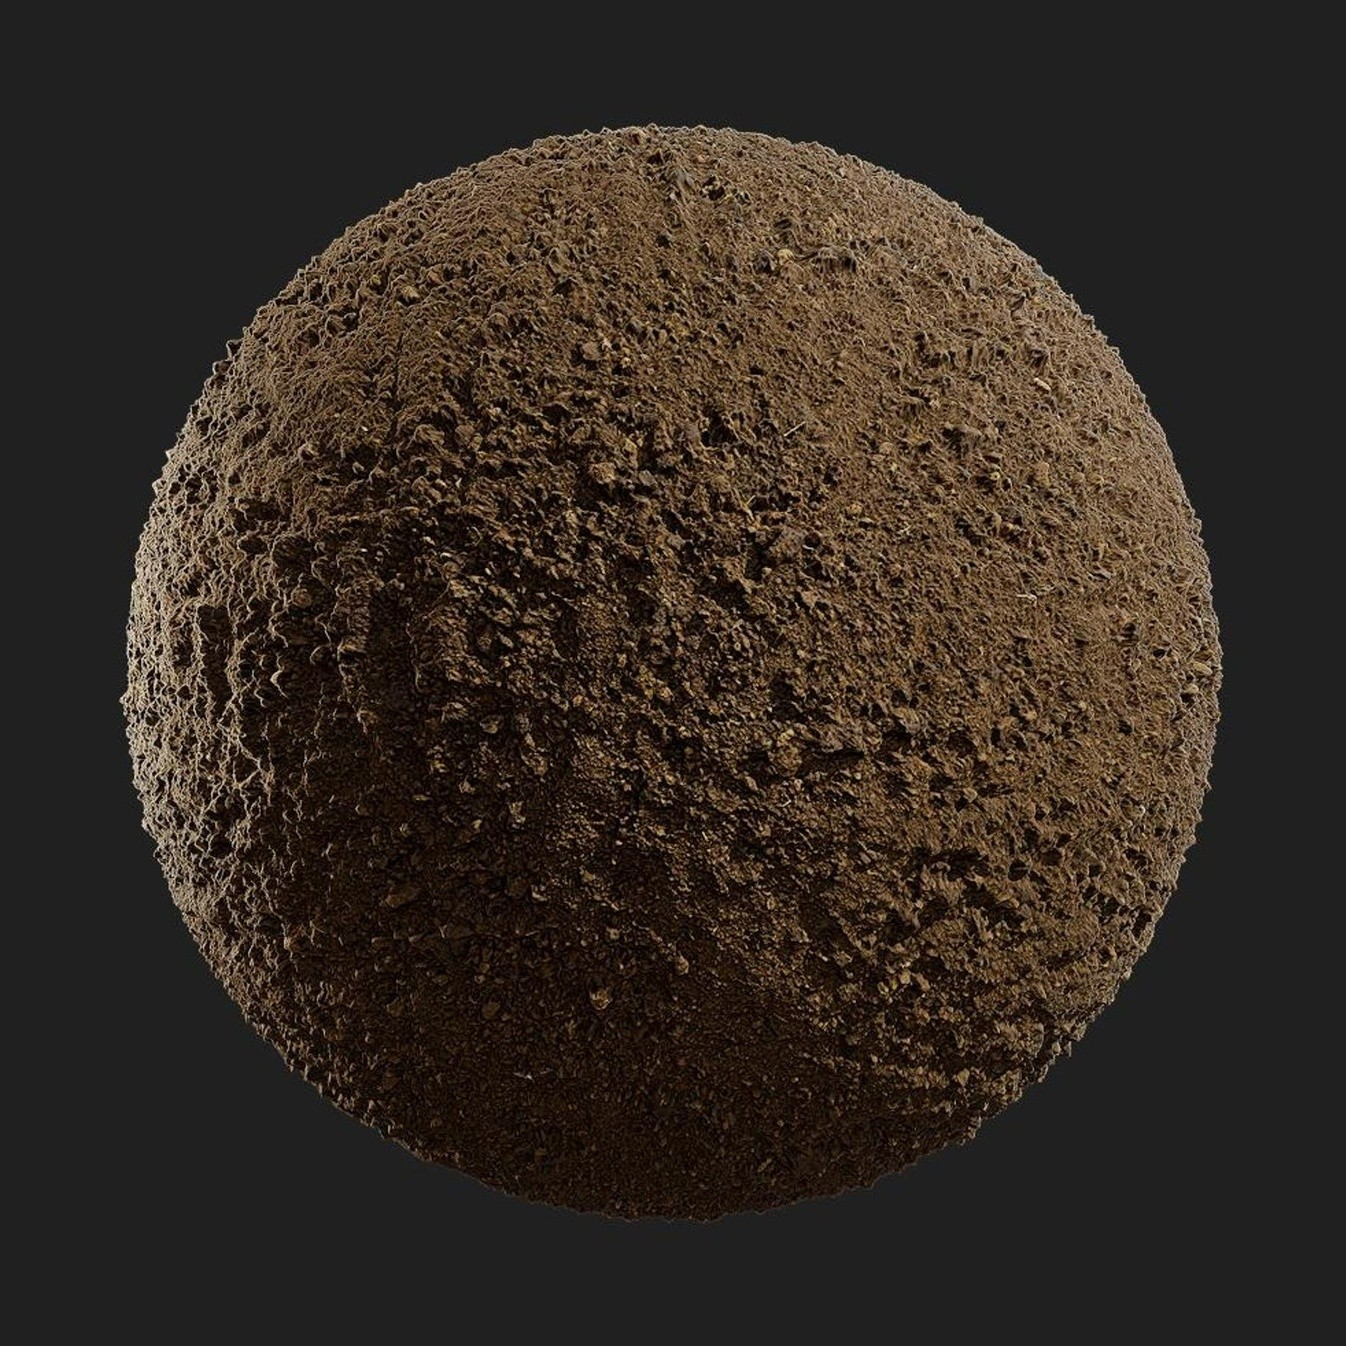
\includegraphics[width=\linewidth]{images/soilmud.jpg}
            \caption{"Soil Mud" material}
        \end{subfigure}
        \hfill 
        \begin{subfigure}{0.48\linewidth}
            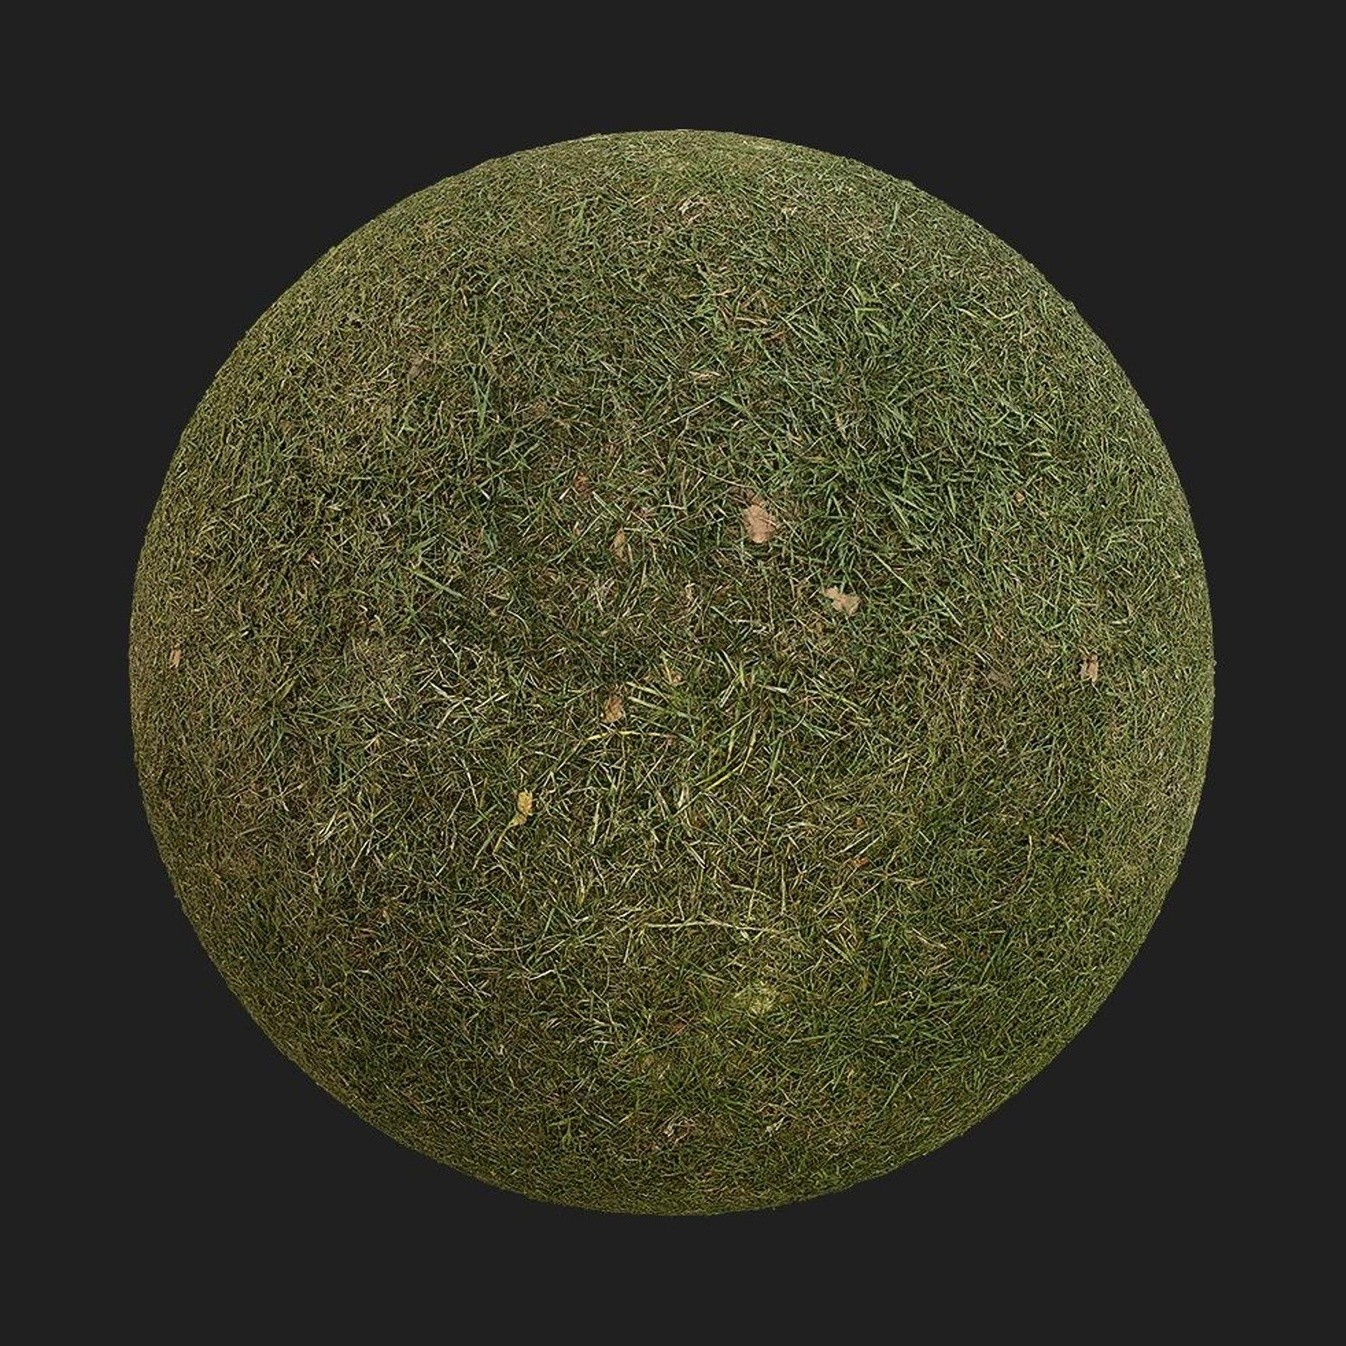
\includegraphics[width=\linewidth]{images/grass.jpg}
            \caption{"Lawn Grass" Material}
        \end{subfigure}
        
        \vspace{1em}
        
        \begin{subfigure}{\linewidth}
            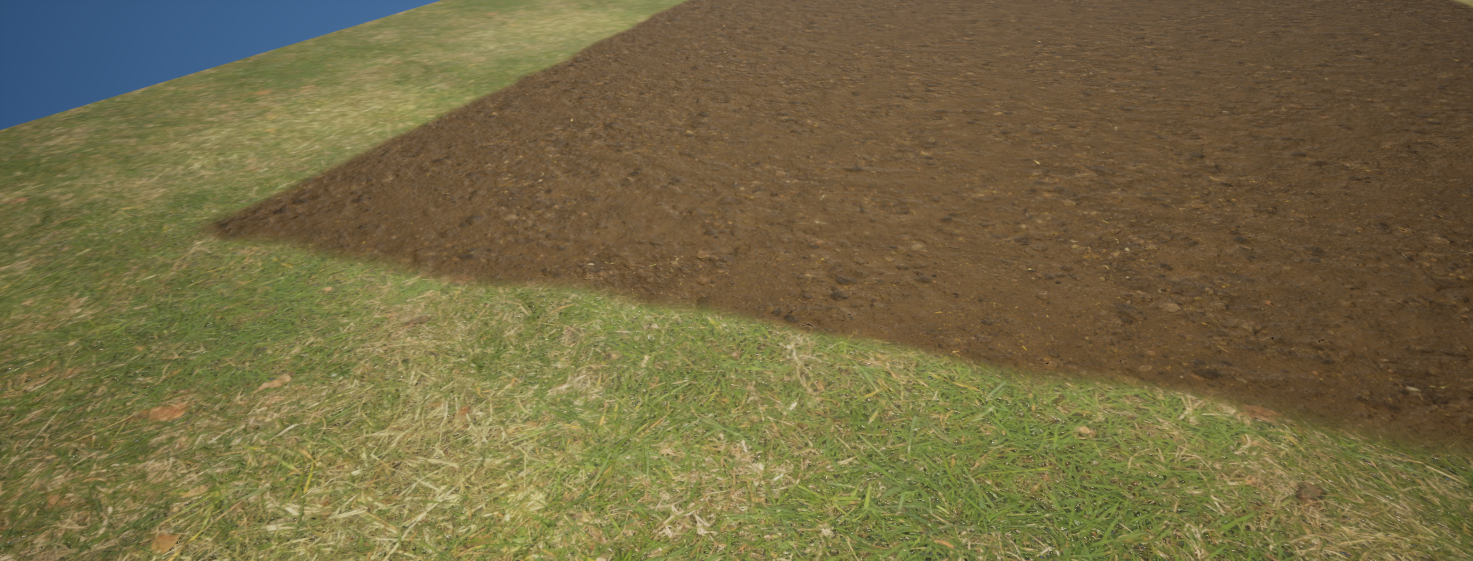
\includegraphics[width=\linewidth]{images/blendedground.png}
            \caption{Landscape actor with blended-ground material applied}
        \end{subfigure}
        
        \caption{The materials used for the digital twin's terrain, both isolated and combined.}
        \label{mat-blend}
        
    \end{minipage}
    
\end{figure}

\subsubsection{Materials}

For the terrain within the crop field, I used ”Soil Mud” \cite{quixel_soil_mud_fab}, signifying the existence of bare soil and crop vegetation, while for the surrounding area I used ”Lawn Grass” \cite{quixel_lawn_grass_fab}, simulating short grass. Unreal Engine allows further processing of the selected materials, enabling the display of several different variations of the same scene. Specifically,  by introducing weights to the texture components that define each material, the ground can be more or less reflective by altering its roughness, implying different levels of moisture present, along with the overall surface brightness, by adjusting the respective RGB intensity values. I exposed the material parameters to UE's interface during the digital twin development for quicker and more intuitive access but did not alter them during the data accumulation.

Assigning different materials on UE’s Landscape actor was achieved by using material blending. In this context, this process includes creating a multilayer material, enabling different textures to be applied by simply drawing one on top of the other. I manually performed the blending, as the manual painting of the landscape appeared to be a more straightforward yet precise workflow. The applied blended material is illustrated in Figure~\ref{mat-blend}.


\subsubsection{Landmass}

The Landmass Plugin is a procedural tool, designed to edit UE’s Landscape actor \cite{epic_landmass_building_worlds}. Its ability to stochastically shape the ground, creating height variations across it, is particularly relevant, since height differences across the terrain can cast shadows, introducing noise to the measurement of a surface's GRVI. Considering that agricultural fields should be relatively flat, the intensity of the displacement that could be applied is limited. Yet, even for the lower levels of displacement, the impact on the shadows was noticeable (Figure~\ref{landmass-int}).

\begin{figure}[htb]
    \centering
    
    \begin{minipage}{1\textwidth}
    
        \begin{subfigure}{0.32\linewidth}
            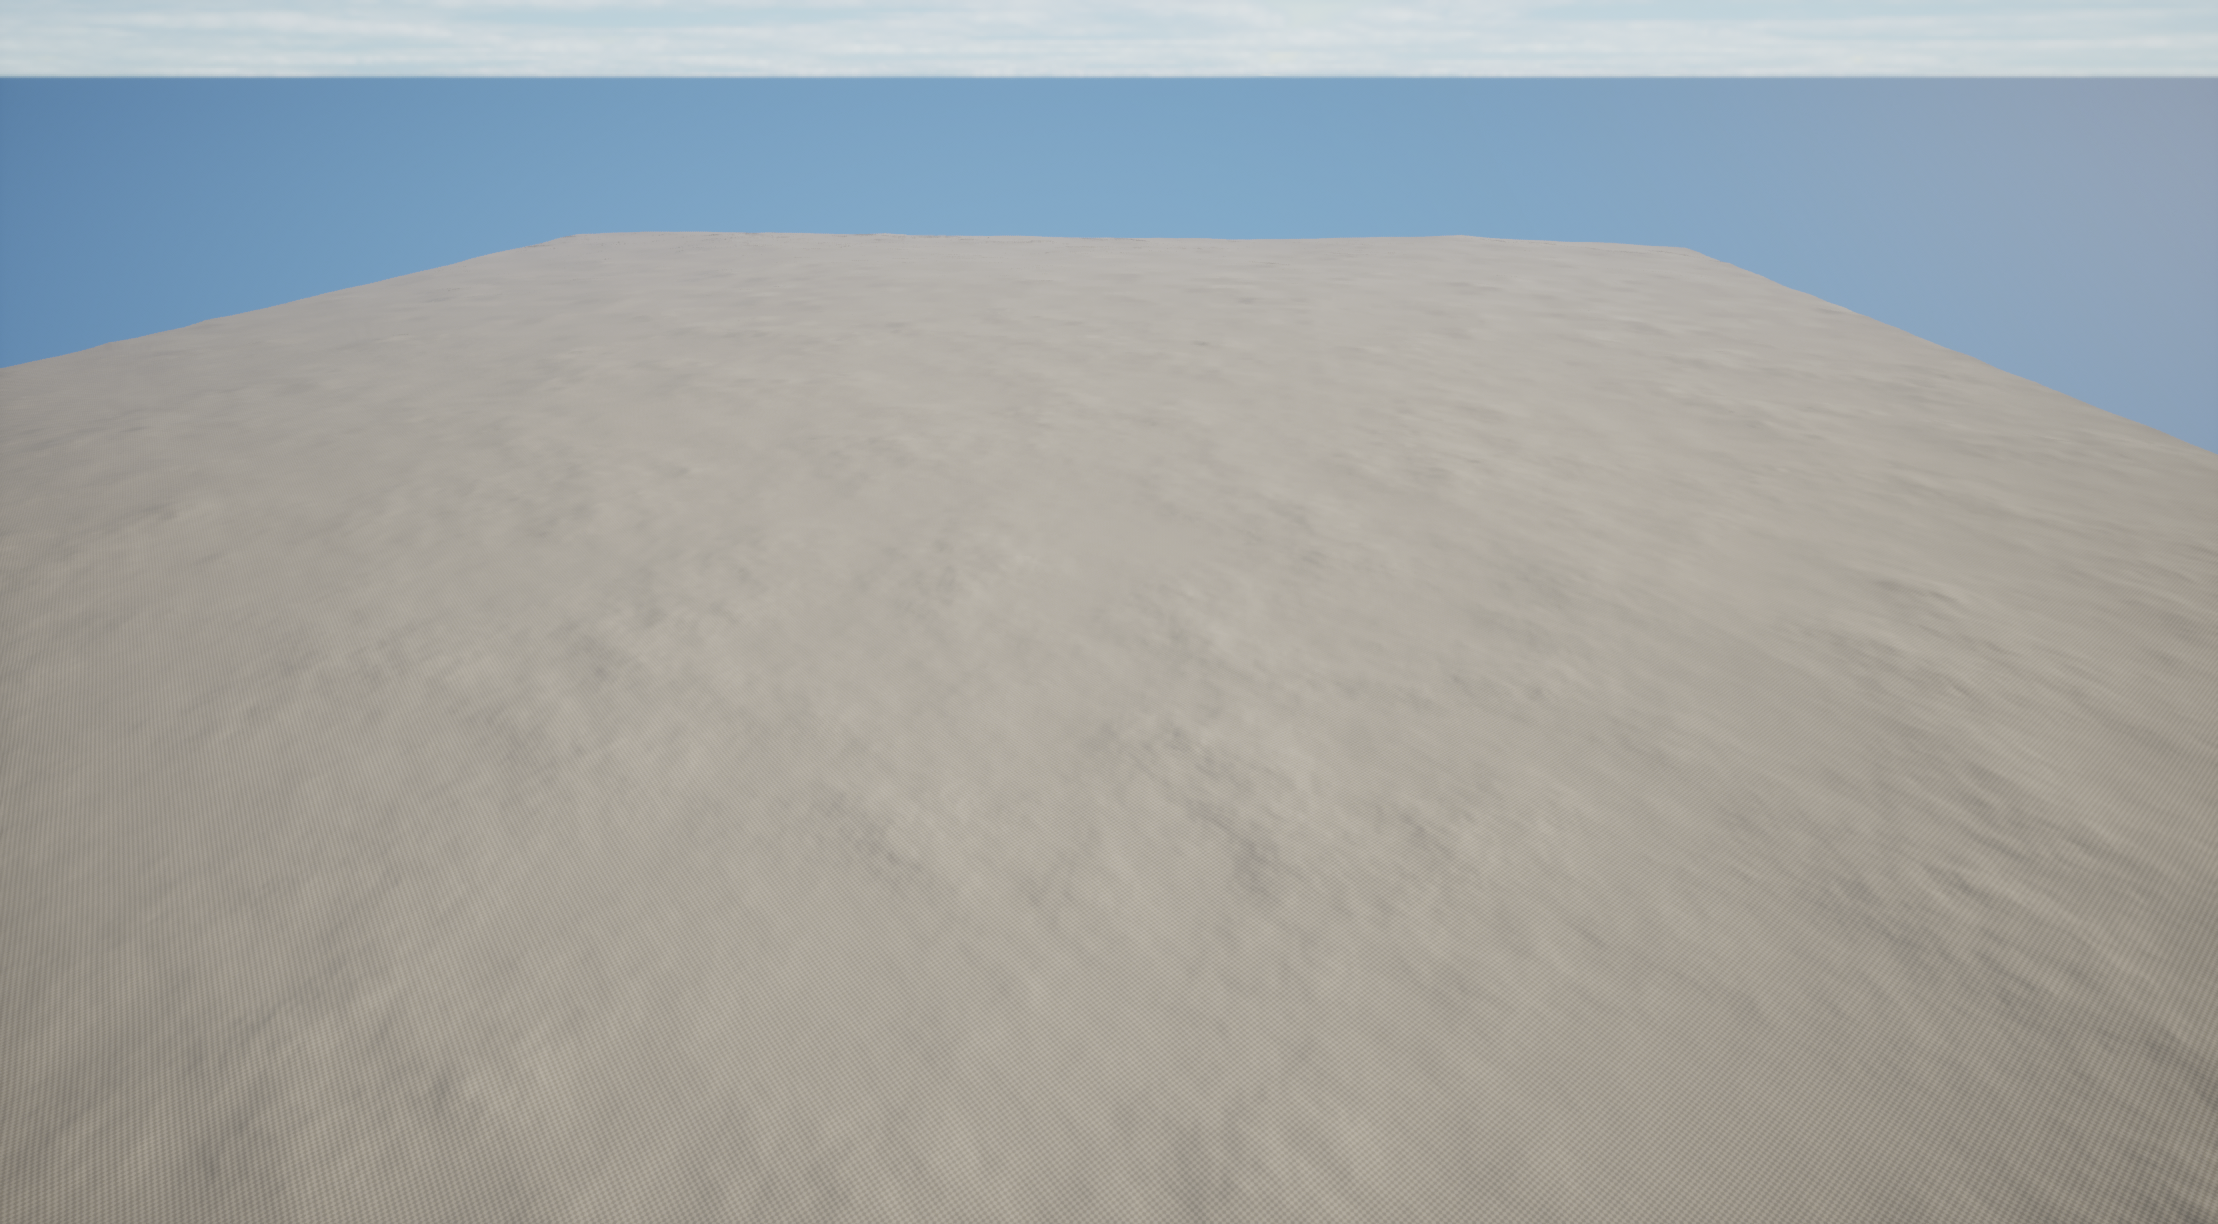
\includegraphics[width=\linewidth]{images/noise600.png}
            \caption{Disp. Height: 600}
        \end{subfigure}\hfill
        \begin{subfigure}{0.32\linewidth}
            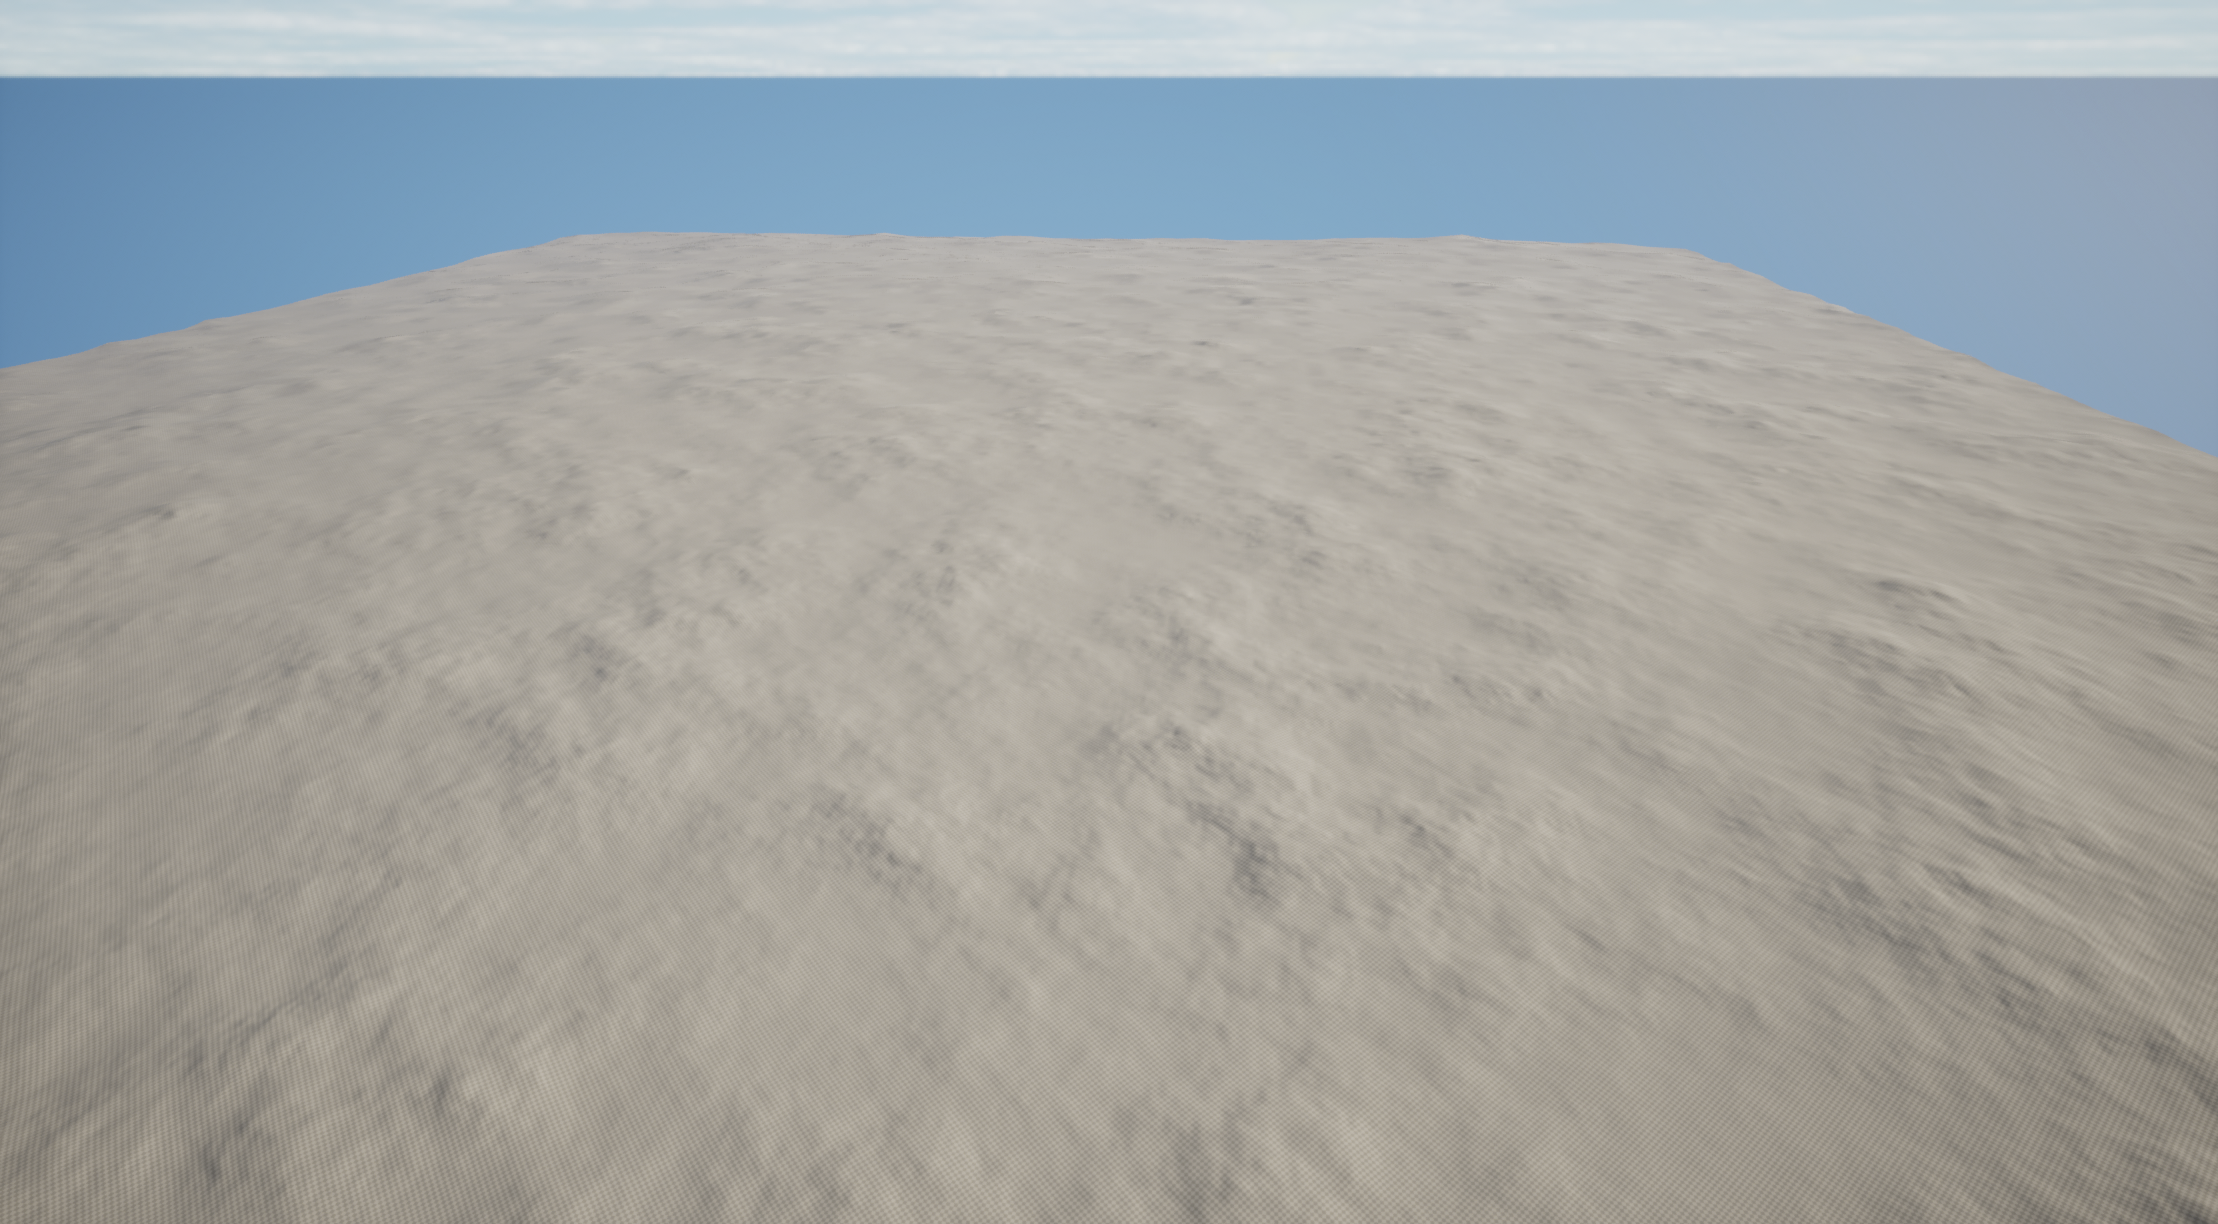
\includegraphics[width=\linewidth]{images/noise1200.png}
            \caption{Disp. Height: 1200}
        \end{subfigure}\hfill
        \begin{subfigure}{0.32\linewidth}
            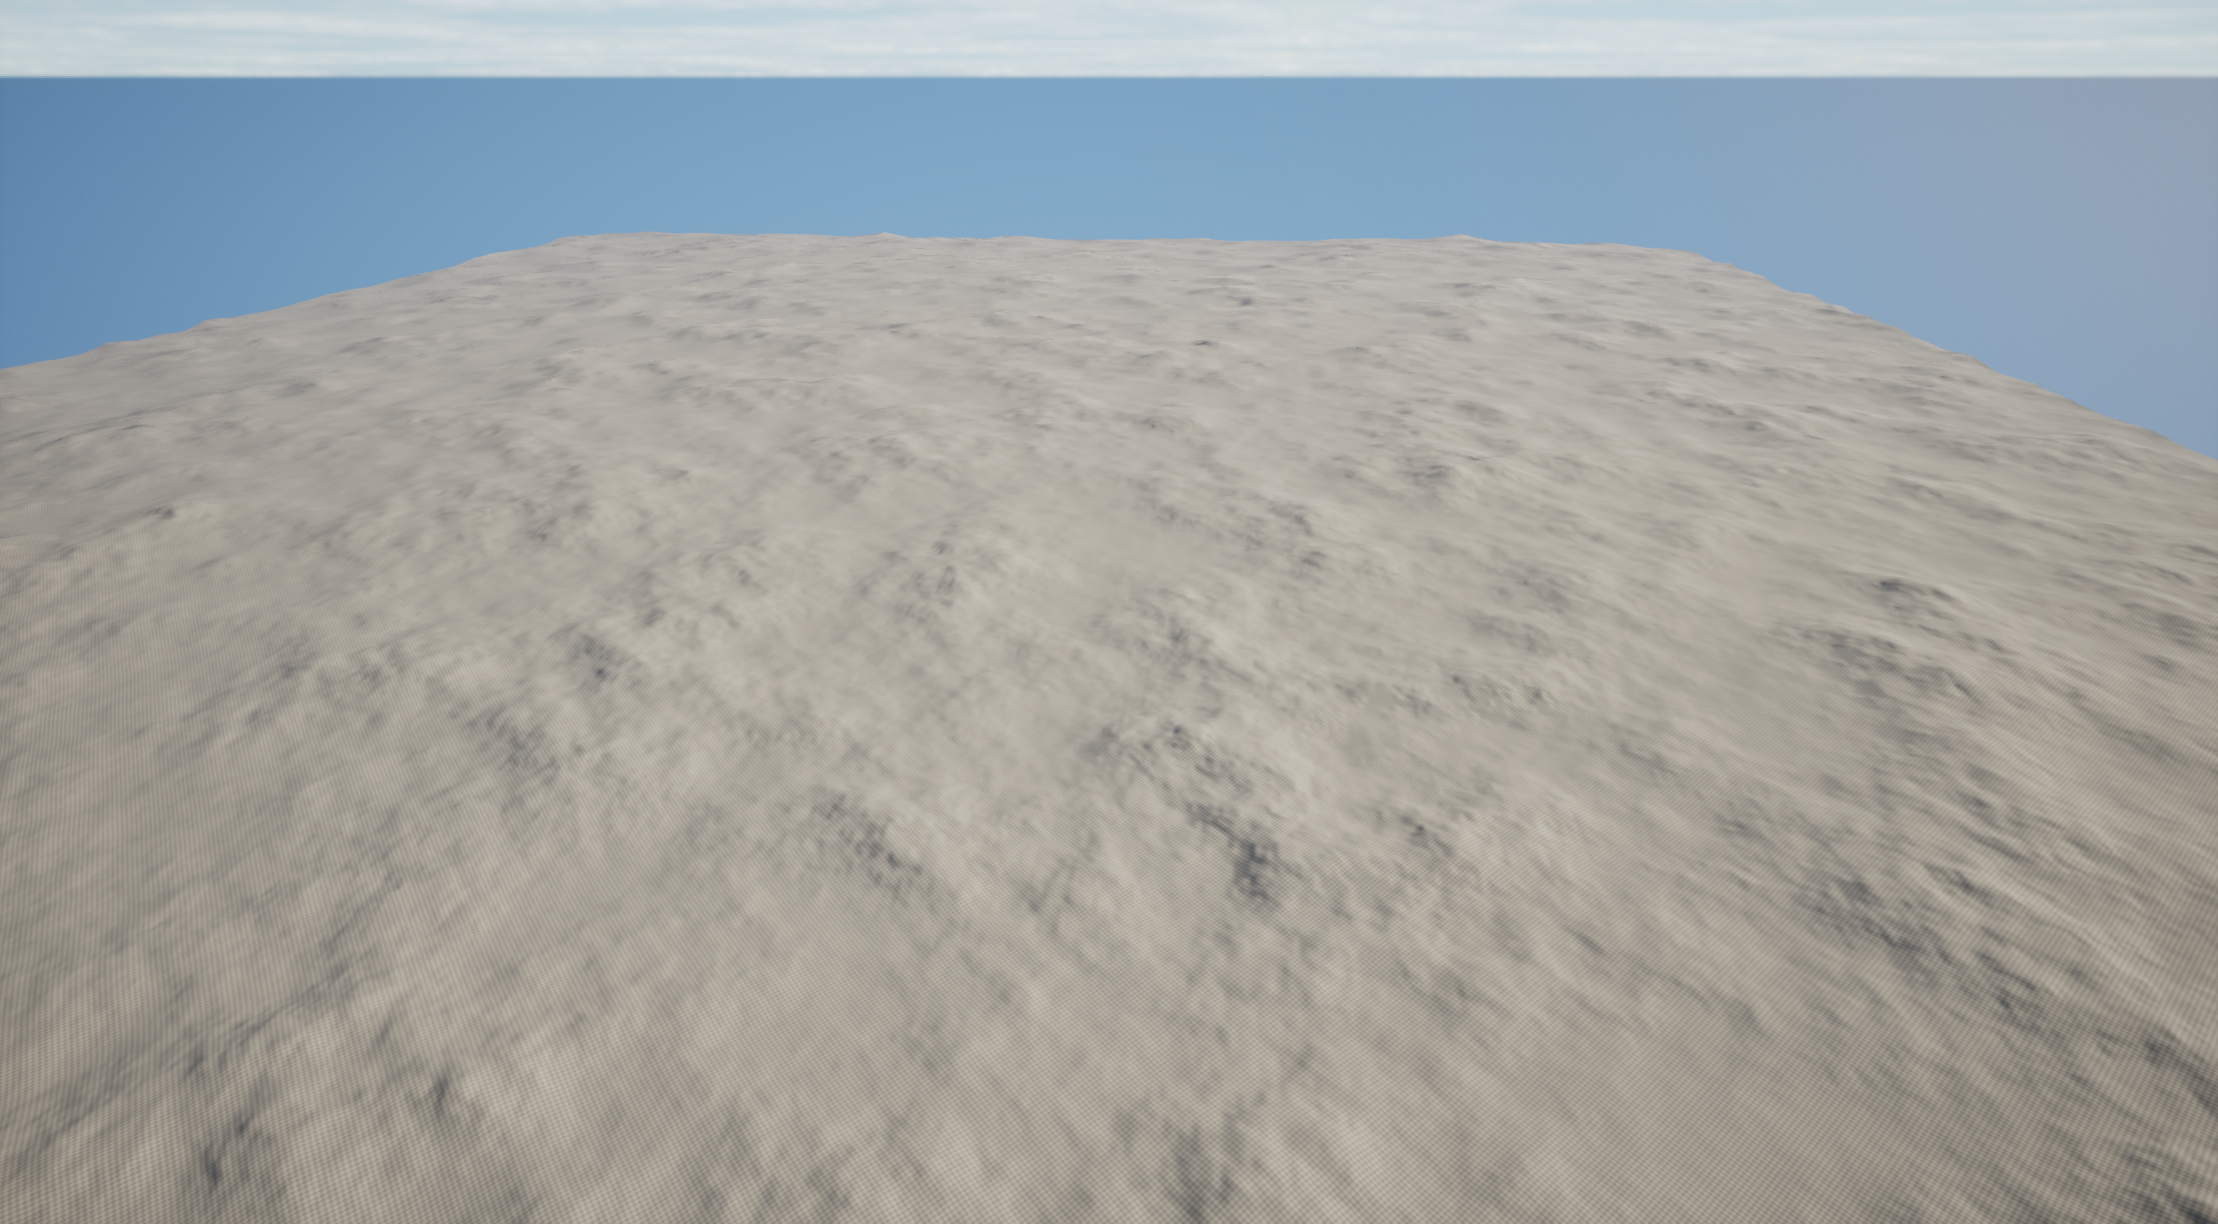
\includegraphics[width=\linewidth]{images/noise1800.png}
            \caption{Disp. Height: 1800}
        \end{subfigure}
        
        \vspace{1em}
        
        \begin{subfigure}{\linewidth}
            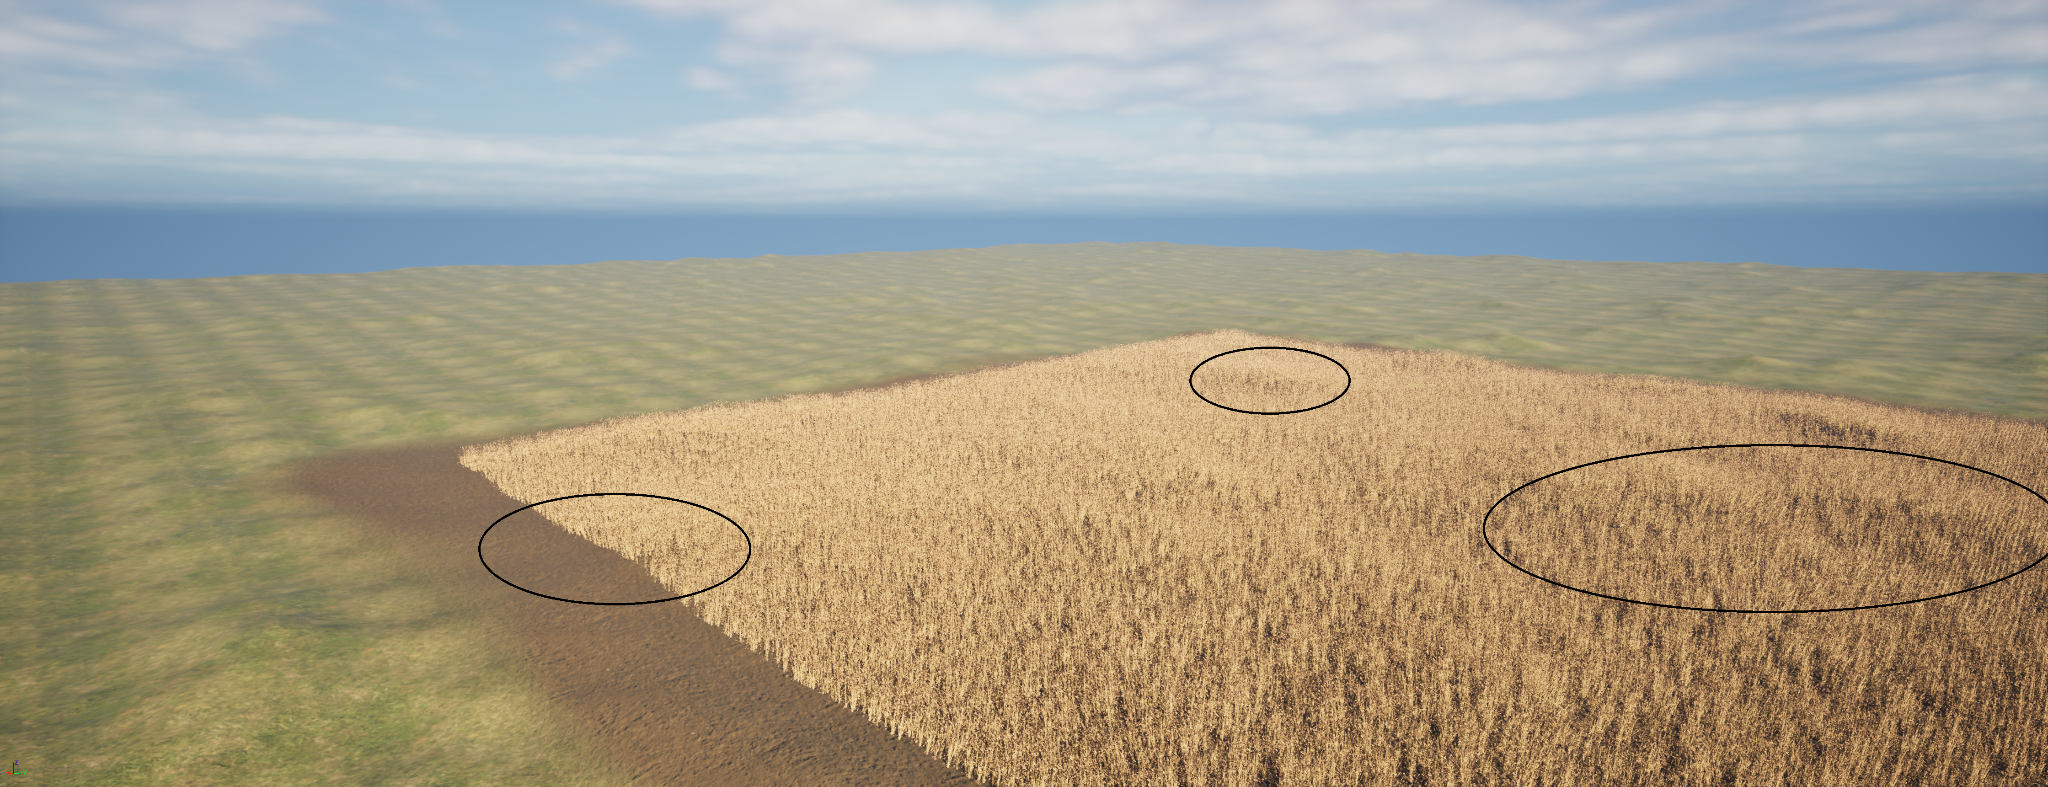
\includegraphics[width=\linewidth]{images/HighresScreenshot00002_4MB.png}
            \caption{Rendered scene with heavy terrain displacement applied. The encircled areas point out several cases of terrain curvature and its consequent effect on cast shadows upon the field canopy.}
        \end{subfigure}
        
        \caption{Using landmass to simulate terrain displacement. The "Displacement Height" parameter arranges the intensity of the terrain displacement, with  the new highest point of the terrain being half of the "Displacement Height" units above 0 and the lowest being half of the "Displacement Height" below 0.}
        \label{landmass-int}
        
    \end{minipage}
\end{figure}
    
Eventually, no data were captured with any amount of displacement, as I did not identify any efficient way for measuring illuminance in parts of the field that were shaded by the simulated short hills and valleys. However, capturing these cases remains a strong objective for the future. With the establishment of a reliable measuring method, the robustness of the trained model will be increased by their inclusion.

\subsection{Plants Generation}
The next step in the digital twin development was the generation of the crop vegetation. I selected wheat as the simulated crop species, as its dense planting structure forms a continuous canopy, suitable for observing its property of distributing reflected light unevenly. This assumption was later verified, since there were significant variations in the photometric quantities measured in the scene depending on the solar zenith angle.

The mesh I used was ”Wheat Grass” \cite{quixel_wheat_grass_fab}. I slightly adjusted its material's stock color to a warmer tone, enhancing the perceived realism of the simulation. This mesh also included a wind simulation by default, but I manually removed it to ensure that the camera captures the same scenes with each render, with the lighting conditions being the only varying factor.

\subsubsection{Procedural Content Generation}

The Procedural Content Generation (PCG) framework allows the developer to define rules for the procedural placement of assets \cite{epic_pcg_overview}. It samples the terrain and provides both the ability to place static meshes stochastically within bounds or organized in grids, with specific distances between them. I found the latter particularly useful for reducing the time needed to simulate the typical appearance of a field, since by using PCG, vegetation can be generated automatically while maintaining precision.

There were two contradicting factors affecting the organization of the meshes that represent wheat stalks. On the one hand, the plants have to be spatially organized, simulating the process of being artificially planted by specialized machinery. On the other hand, the strictly grid-based placement of wheat stalks leads to a very unnatural appearance. To tackle this, I decided that meshes would be placed on a grid, and randomness could be introduced to the scale and rotation of each mesh. Noise was also introduced to the modeled vegetation’s density, by allowing several grid cells to remain empty. The inclusion of these factors led to a sufficiently natural look.

The resulting model can be seen in Figure~\ref{pcg-field}. It can be observed that the wheat meshes are placed in an organized grid rather than completely stochastically. The introduced noise pertains to its rotation, height difference, and planting density.

\begin{figure}[htb]
    \centering
    
    \begin{subfigure}{0.48\linewidth}
        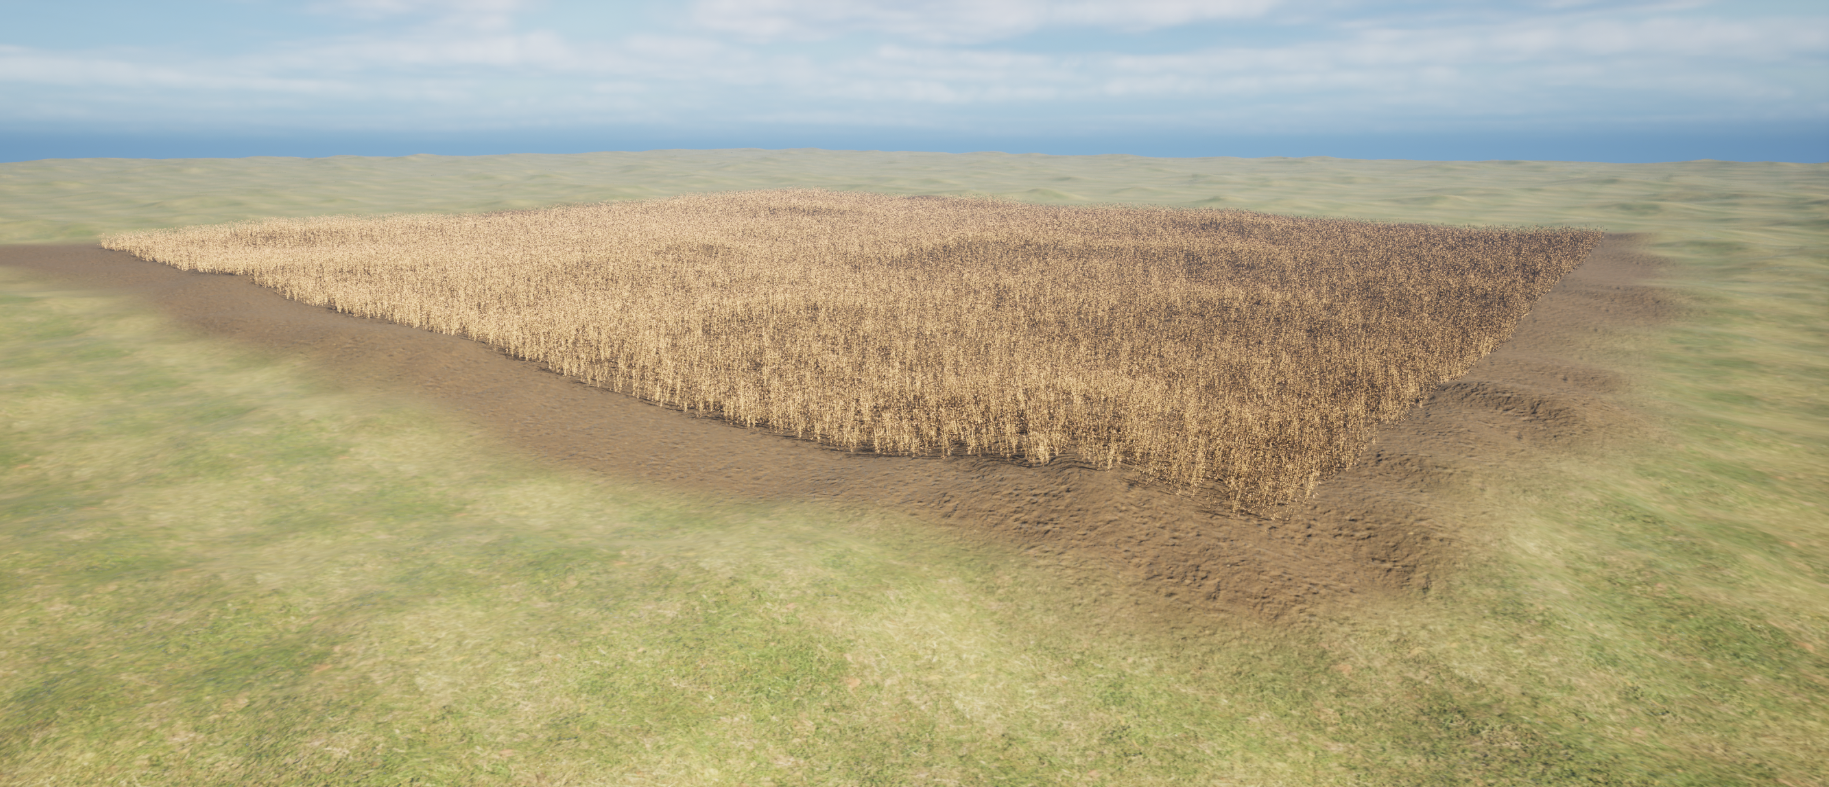
\includegraphics[width=\linewidth]{images/wheat-field.png}
        \caption{Image of the generated wheat field from the side.}
    \end{subfigure}\hfill
    \begin{subfigure}{0.48\linewidth}
        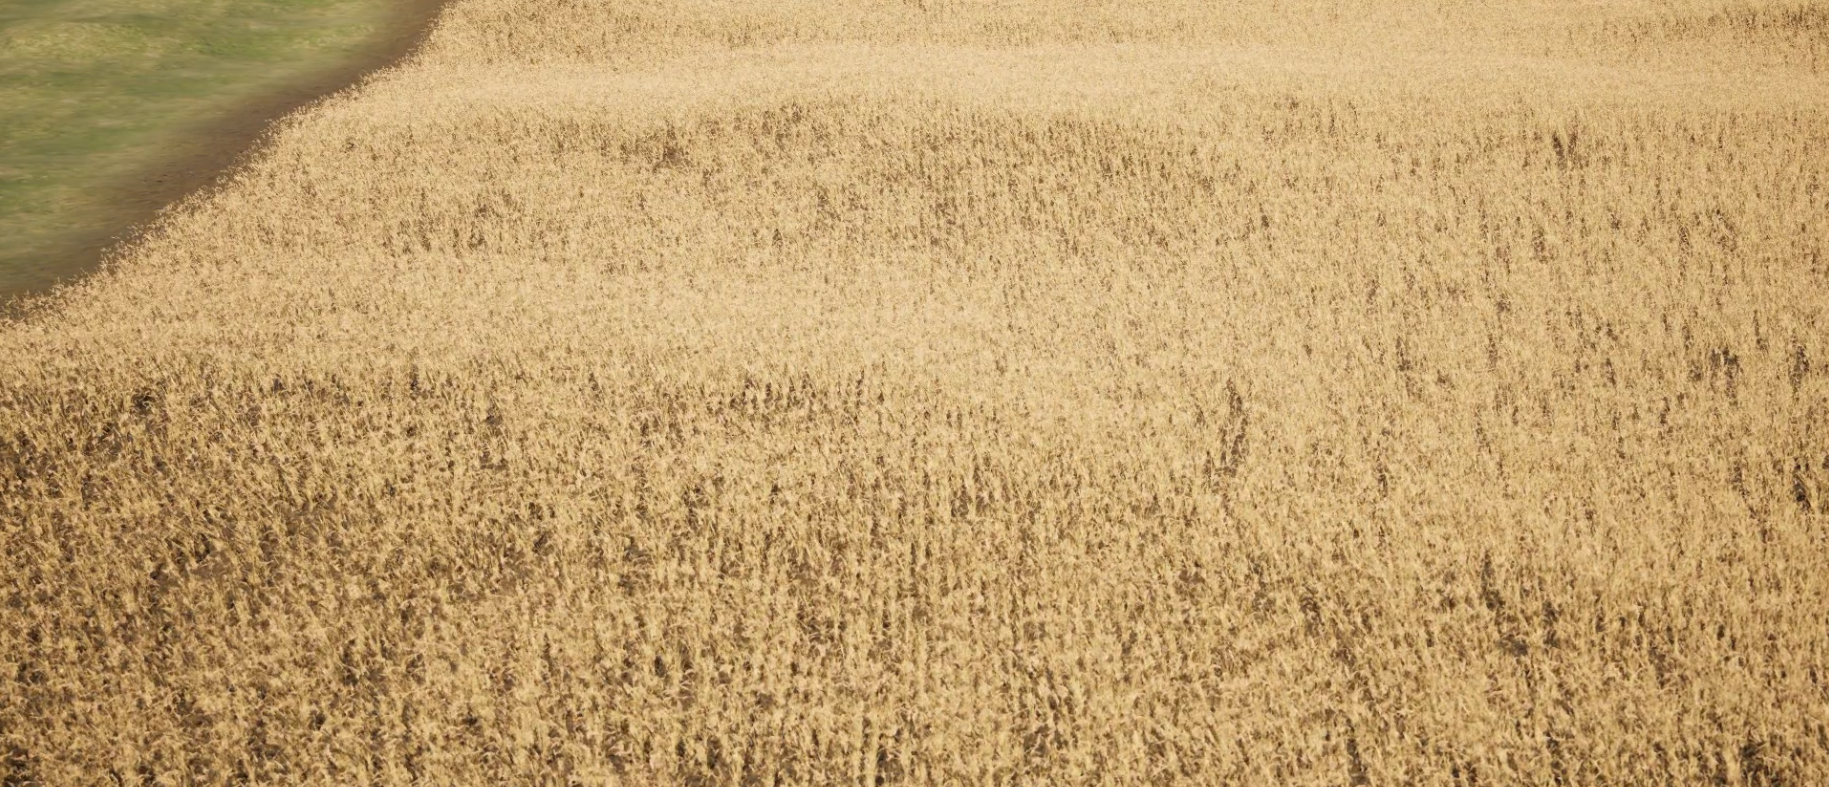
\includegraphics[width=\linewidth]{images/wheat-above.png}
        \caption{Image of the generated wheat field from above.}
    \end{subfigure}
    
    \caption{Images of wheat generated using the Procedural Content Generation tool.}
    \label{pcg-field}
\end{figure}

\subsubsection{Different Plant Materials}

So far, all the vegetation meshes inserted into the scene were sharing the same slightly altered stock material. The final part of the plants generation process was the introduction of variability to the material of the plants across the field. There were two main motives behind this addition. Firstly, this way the realism of the rendered scene is enhanced, considering that, in a real world field, the color of the crops varies due to different growth stages, hydration state, influence of a disease and more. The second motive was enlarging the diversity of the training examples. Specifically, by making the red and green band reflectance change from plant to plant in the field, the trained model becomes more robust, learning the relationships between the measured and ground truth GRVI values for more than one possible cases. It is also important to mention that, as described in more detail later on, measured GRVI appears to behave differently depending on the original GRVI of the material and the illumination conditions. This also affected the robustness of the model.

In order to simulate these differences in the reflectance of plants across the field, I developed a GRVI map, indicating the appropriate value for each part of it. To ensure a degree of realism, I used a GRVI map conceived by aerial images of an actual field (!!!!!!!!!!!!!!!! i cannot find the original publication!!!!) as the basis. Although the field studied in this work was not a wheat field, I determined that the GRVI values present in this map do appear to be realistic for lush wheat. A part of the selected GRVI map that fitted the dimensions of the simulated field was selected.

\begin{figure} [htb]
    \centering
    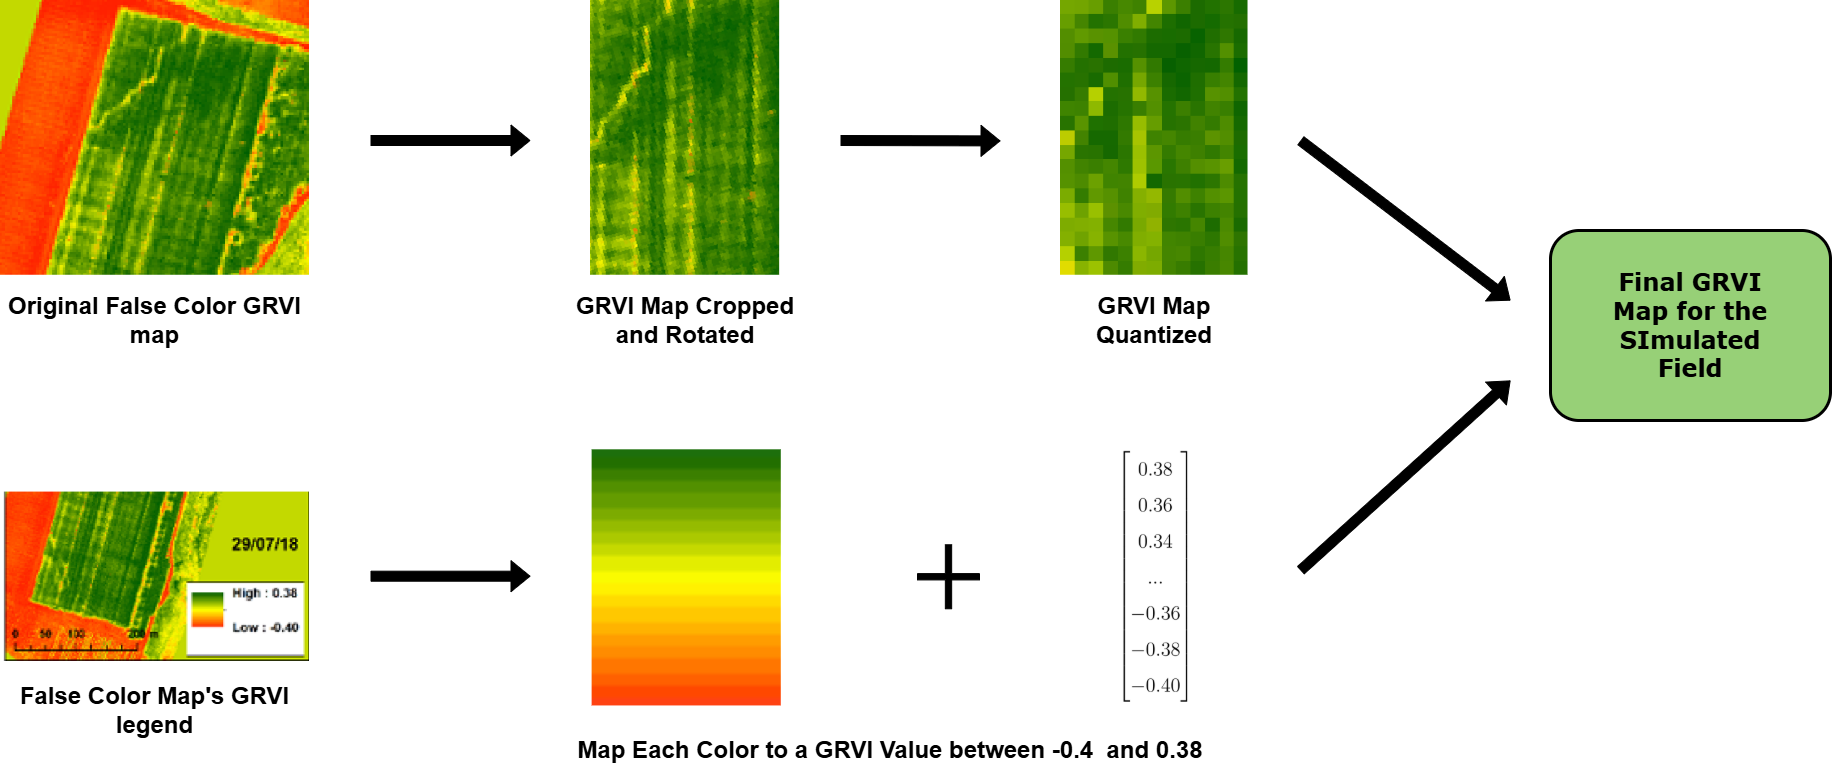
\includegraphics[width=1\linewidth]{images/grvimap.png}
    \caption{Process of creating a GRVI map for the materials assigned to the simulated field, using a real-world GRVI map as a baseline.}
    \label{grvimap}
\end{figure}

The original segment of the map was a 195 by 210 grid, with each cell representing one of 39 discrete GRVI values - identified after processing the legend of the original image. Since the reflectance assignment to the different parts of the field would have to be done either manually or the whole structure of the plant mesh generation would have to be restructured and developed as a C++ class, I avoided the exact recreation of this grid. Instead, I quantized the map using a 15 by 15 median filter, resulting in a 13 by 14 grid. Using the legend provided in the original false color map, it was possible to assign GRVI values to parts of the field based on their corresponding region in the quantized GRVI map (Figure~\ref{grvimap}). Eventually, I saved the GRVI map as a CSV file, each cell of which represented the average GRVI of the material assigned to the respective part of the field. Importantly, this is the GRVI of the material's texture, as it is applied to the meshes. When measured in the simulated environment under diffuse light conditions, due to the presence of soil and errors stemming from the calculation methods, GRVI appeared different.

Following the finalization of the GRVI map, I divided the simulated field into 1.9 by 1.9 meter segments, arranged  in the aforementioned 13 by 14 grid. Each field segment corresponded to one cell of the created CSV and was assigned the GRVI value associated with that cell. Table~\ref{tab_grvi_map} presents the GRVI values assigned to each segment, with its rows and columns corresponding to the spatial rows and columns of the simulated field, respectively. Figure~\ref{diff-griv-field} illustrates the final result of the assignment.

\begin{table}[H]
\centering
\scriptsize
\caption{Analytical table of GRVI values assigned to each part of the field.}
\label{tab_grvi_map}
\resizebox{\textwidth}{!}{%
\begin{tabular}{ccccccccccccc}
\hline
C1 & C2 & C3 & C4 & C5 & C6 & C7 & C8 & C9 & C10 & C11 & C12 & C13 \\
\hline
0.20 & 0.20 & 0.22 & 0.32 & 0.30 & 0.30 & 0.10 & 0.24 & 0.32 & 0.36 & 0.34 & 0.34 & 0.36 \\
0.22 & 0.30 & 0.34 & 0.34 & 0.28 & 0.18 & 0.30 & 0.36 & 0.38 & 0.36 & 0.36 & 0.34 & 0.36 \\
0.26 & 0.24 & 0.26 & 0.26 & 0.32 & 0.32 & 0.36 & 0.36 & 0.36 & 0.38 & 0.36 & 0.34 & 0.36 \\
0.28 & 0.32 & 0.36 & 0.26 & 0.34 & 0.34 & 0.36 & 0.36 & 0.38 & 0.38 & 0.34 & 0.26 & 0.36 \\
0.32 & 0.34 & 0.34 & 0.36 & 0.36 & 0.26 & 0.32 & 0.38 & 0.38 & 0.36 & 0.36 & 0.32 & 0.38 \\
0.34 & 0.34 & 0.36 & 0.28 & 0.36 & 0.20 & 0.30 & 0.36 & 0.38 & 0.36 & 0.32 & 0.30 & 0.36 \\
0.34 & 0.32 & 0.10 & 0.34 & 0.34 & 0.16 & 0.26 & 0.36 & 0.36 & 0.36 & 0.26 & 0.28 & 0.34 \\
0.30 & 0.30 & 0.16 & 0.36 & 0.34 & 0.32 & 0.26 & 0.34 & 0.32 & 0.34 & 0.30 & 0.32 & 0.38 \\
0.34 & 0.26 & 0.36 & 0.36 & 0.34 & 0.14 & 0.22 & 0.34 & 0.34 & 0.30 & 0.32 & 0.28 & 0.36 \\
0.08 & 0.30 & 0.36 & 0.36 & 0.32 & 0.12 & 0.30 & 0.30 & 0.32 & 0.32 & 0.26 & 0.28 & 0.36 \\
0.20 & 0.34 & 0.34 & 0.36 & 0.34 & 0.14 & 0.24 & 0.32 & 0.30 & 0.30 & 0.32 & 0.30 & 0.36 \\
0.26 & 0.30 & 0.32 & 0.30 & 0.34 & 0.14 & 0.26 & 0.34 & 0.30 & 0.26 & 0.26 & 0.22 & 0.36 \\
0.26 & 0.28 & 0.22 & 0.30 & 0.30 & 0.10 & 0.36 & 0.34 & 0.34 & 0.36 & 0.34 & 0.28 & 0.34 \\
0.20 & 0.32 & 0.24 & 0.26 & 0.30 & 0.18 & 0.16 & 0.32 & 0.28 & 0.30 & 0.26 & 0.26 & 0.34 \\
\hline
\end{tabular}%
}
\end{table}

\begin{figure} [htb]
    \centering
    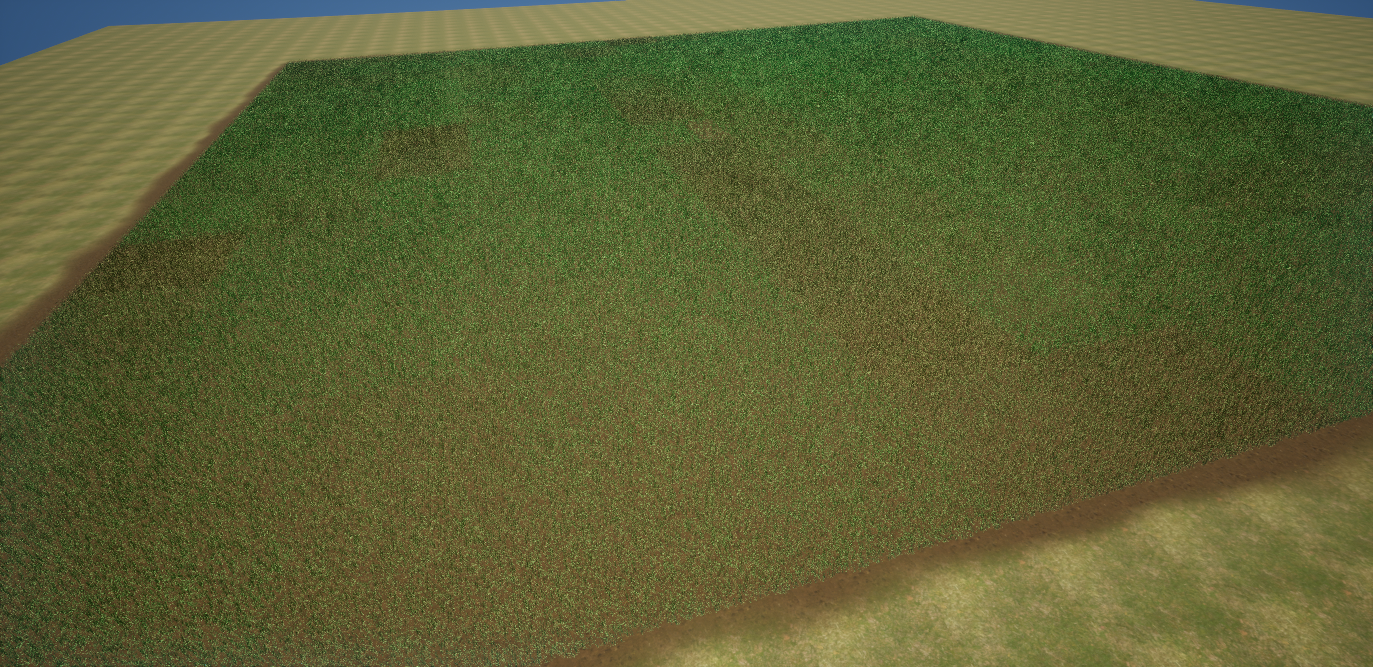
\includegraphics[width=1\linewidth]{images/HighresScreenshot00007.png}
    \caption{Digital twin after different values of inherent GRVI have been assigned to each part of the field, with each discreet segment being a 1900 by 1900 unit square.}
    \label{diff-griv-field}
\end{figure}

\subsection{Tree Meshes}

Illumination variability does not always originate solely from the position and intensity of the light source. The existence of obstacles between the light source and the studied surface do alter the illuminance reaching the surface too, and, consequently, the luminance reflected towards the sensor. Again, this would not affect the calculation of reflectance, assuming that the sensors used and the studied surface were ideal. In the studied case though, I treat shadows as one of the challenges the proposed algorithm aims to address.

An organic way to introduce shadows into the scene is to add trees to it. The objective was for the trees' crowns to cast shadows onto the simulated crops' canopy. Ideally, the created shadows do not occlude the whole field but rather parts of it. This way, by changing the solar zenith angle (SZA), the direction of the shadows changes, also changing the parts of the field that are shaded. The library of tree meshes I selected for this digital twin was \cite{european_hornbeam}. Specifically, the "FT\_EuropeanHornbeam\_Field\_02\_PP" mesh was used. Considering that only a numerable amount of meshes had to be added to achieve the desired result, and in a way that their trunks are not included in the areas of interest of the captured frames, I manually placed them using UE's Foliage Tool \cite{epicgames_foliagetool}. Figure~\ref{tsas} depicts the digital twin post the addition of tree meshes. Specifically, Figures~\ref{ts--104} and \ref{ts-104} show the difference in the shadows' directionality caused by SZA variations.

\begin{figure}[htb]
    \centering
    
    \begin{minipage}{1\textwidth}

        \begin{subfigure}{\linewidth}
            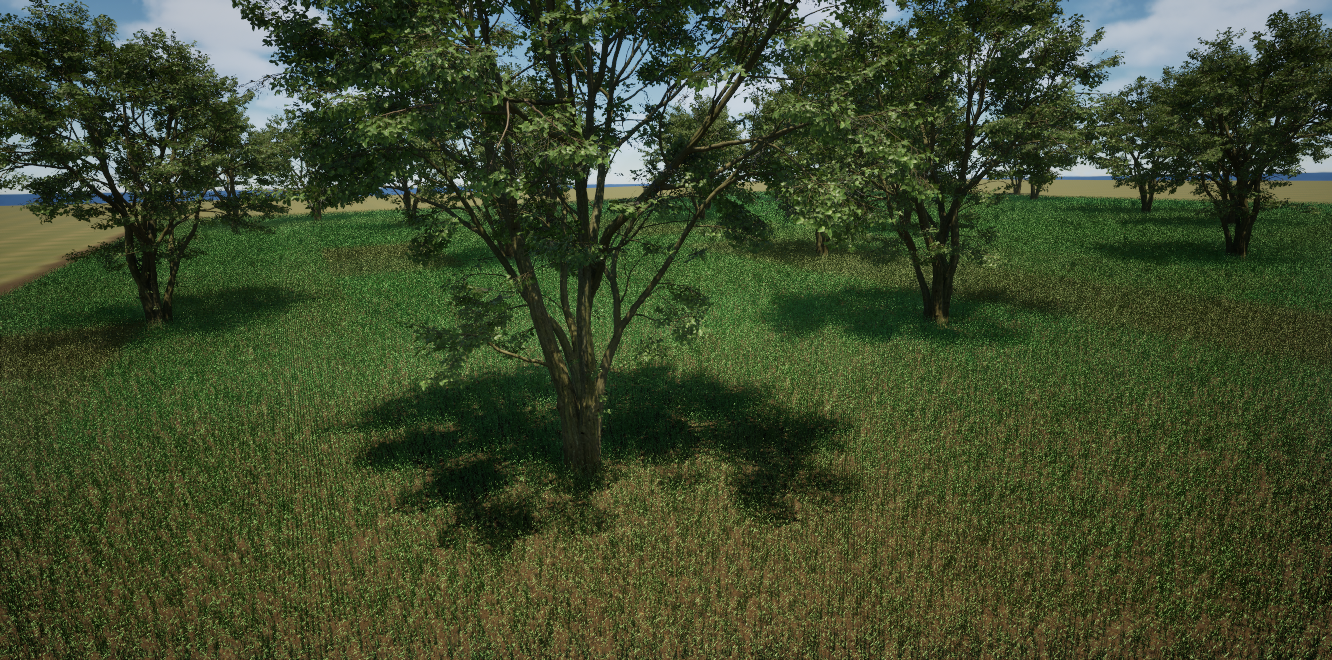
\includegraphics[width=\linewidth]{images/trees-generic.png}
            \caption{Trees added to the digital twin.}
        \end{subfigure}

        \vspace{1em}
    
        \begin{subfigure}{0.48\linewidth}
            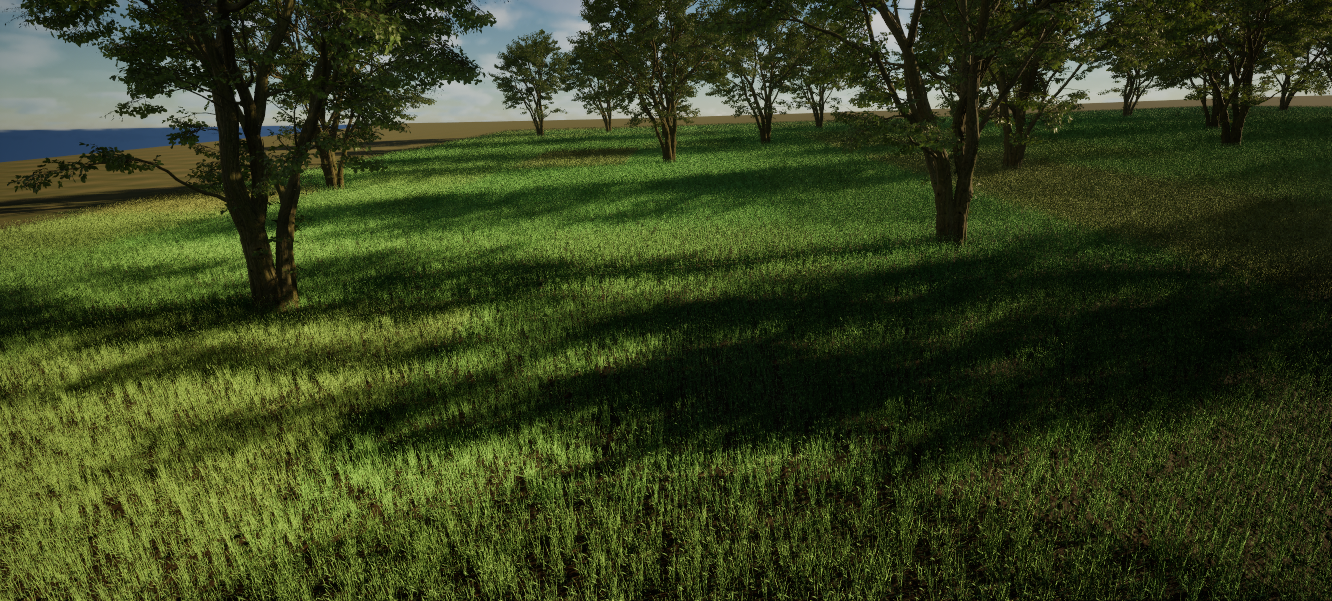
\includegraphics[width=\linewidth]{images/trees-6am.png}
            \caption{Trees' shadows for SZA $ = -104^\circ$}
            \label{ts--104}
        \end{subfigure}
        \hfill 
        \begin{subfigure}{0.48\linewidth}
            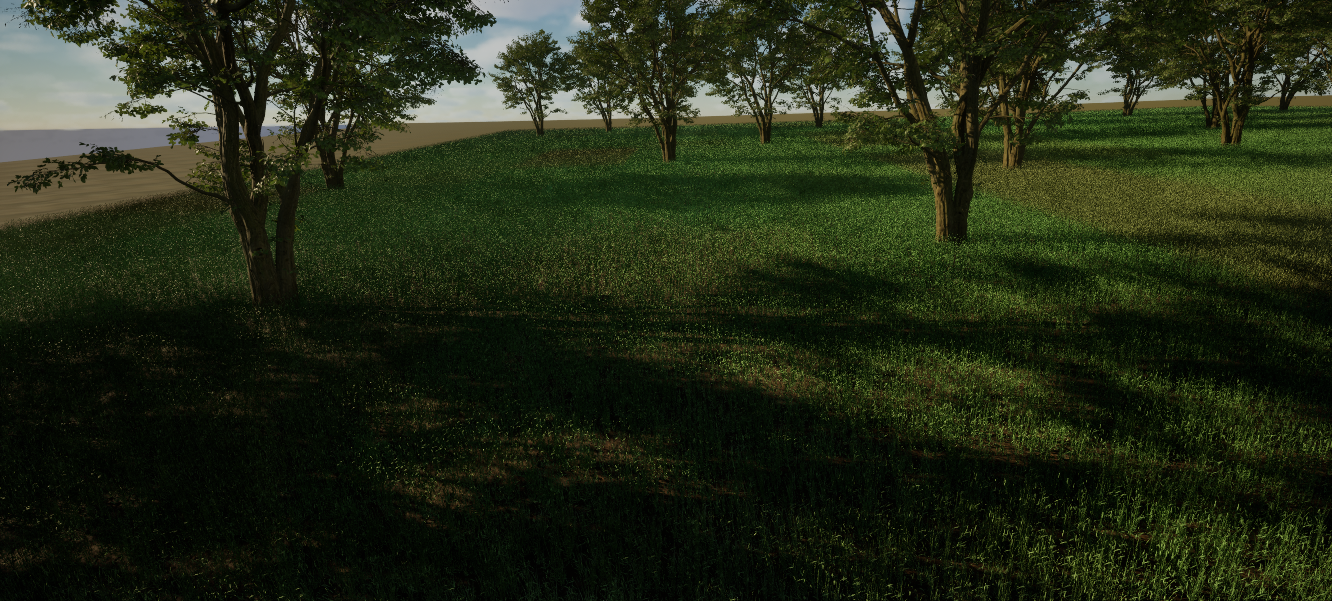
\includegraphics[width=\linewidth]{images/trees-1715.png}
            \caption{Trees' shadows for SZA $ = 104^\circ$}
            \label{ts-104}
        \end{subfigure}        

        
        \caption{Trees added to the digital twin, introducing shadows to parts of the field's canopy. The shaded parts change as the SZA changes, ensuring diversity in the training examples.}
        \label{tsas}
        
    \end{minipage}
    
\end{figure}

\subsection{Lighting Configuration}

The main lighting actors in UE are:

\begin{itemize}
    \item \textbf{Point Light}: Light source similar to a light bulb
    \item \textbf{Spot Light}: Projects light in a cone shape, like a spotlight
    \item \textbf{Rect Light}: Similar to photography umbrellas. Projects light in a cone and creates soft shadows 
    \item \textbf{Directional Light}: Mimics sunlight. Illuminates the whole scene, but its direction determines the behavior of the shadows.
    \item \textbf{Sky Light}: Applies ambient lighting to the scene. Good for simulating outdoor lighting conditions
\end{itemize}

The implemented model contains the last two options, as they are directly suitable for simulating weather phenomena. Directional Light is essential in scenes where the sky is clear, controlling the direction of incident solar radiation and the resulting shadows, while Sky Light is more prominent in scenes with diffuse lighting, where radiative flux is assumed to be incident more uniformly across the scene.

In order to achieve further precision, I manipulated the parameters of Directional Light through the "Sun Position Calculator" plugin. "Sun Position Calculator" can be used for setting the appropriate roll, pitch, and yaw values of the light source, corresponding to the solar position for a specified time and set of geographical coordinates. As a result, the simulated lighting conditions can be more realistic than if the degrees were adjusted manually. The plugin also allows adjustments to the Directional Light intensity, enabling the simulation of brighter and darker scenes.


\subsection{Weather Phenomena Simulation}

There were mainly two sky conditions relevant to this study: clear-sky and cloudy-sky. Clear-sky weather represents the challenging case since, as mentioned above, the position of the sun affects the way radiation is reflected by vegetation. I constructed the simulation in a way that allows multiple Directional Light configurations, considering that there was an apparent need for data collected under more than one illumination scenario in order to achieve higher model robustness. The data collected under these various clear-sky illumination configurations later served as the model's inputs and resemble GRVI values calculated with a high degree of error. In contrast, cloudy-sky weather is treated as ideal for the collection of the ground truth data, since the luminance measured in such conditions remains sufficiently invariant for various solar coordinates.

Clear-sky conditions were easier to implement, given that the default configuration of Sun Position Calculator already does simulate this weather state. Optionally, the Volumetric Clouds actor, which can also be included by default during the creation of a new level in Unreal Engine, can be disabled to fully simulate clear sky. However, this actor itself does not affect Directional Light significantly, as it does not cause light scattering or cast additional shadows.

The primary tool I used for replicating cloudy-sky conditions is “Sky Atmosphere”. In Unreal Engine 5, Sky Atmosphere is a system used for the simulation of the atmosphere of a planet. Among the available options, there are parameters for adjusting the atmospheric height and color and, most importantly for this task, the amount of light diffusion and absorption occurring as sunlight enters the atmosphere and comes in contact with its particles. These parameters are named ”Mie Scattering Scale” and ”Mie Absorption Scale”, respectively. In the context of this work, I focused more on experimenting with "Mie Scattering Scale" adjustments, as the objective was to identify a configuration that eliminates the directionality of light without reducing the brightness of the scene. Ultimately, by increasing the intensity of Directional Light and Mie Scattering Scale and decreasing the amount of light absorption, a desirable result was achieved.

Figure~\ref{notclvscl} illustrates the difference between zero and non-zero Mie Scattering Scale applied. In the first case (Figure~\ref{nonfog}), the solar zenith angle (SZA) is set to $56^o$, making the sun closer to the right side of the frame. Consequently, the rightmost half of the field appears less illuminated than the leftmost. When cloudy weather is simulated, though (Figure~\ref{fog}), despite the SZA remaining the same, the illumination unevenness gets mitigated.
 
\begin{figure}[htb]
    \centering
    
    \begin{subfigure}{0.48\linewidth}
        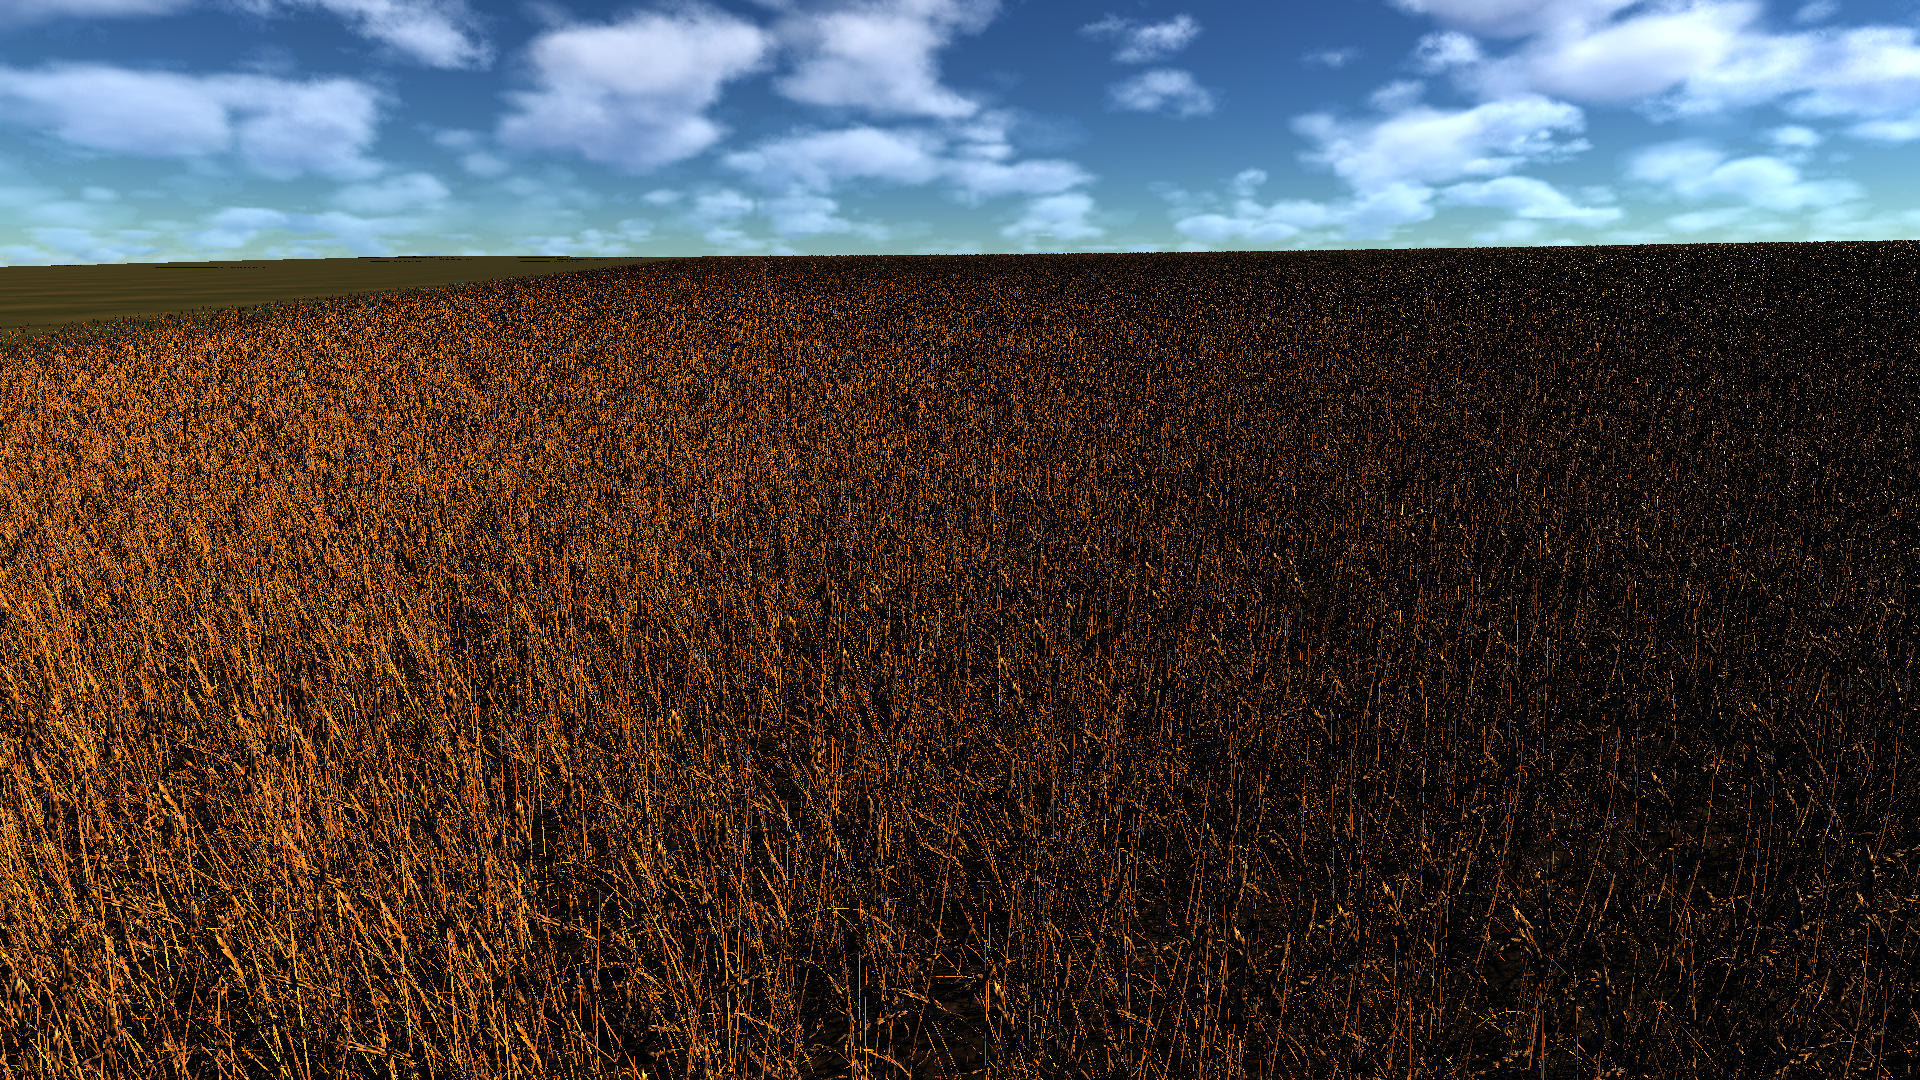
\includegraphics[width=\linewidth]{images/nonfoggy10.png}
        \caption{Field illuminated with the SZA being set to $56^o$ and Mie Scattering Scale being set to its default value (near zero).}
        \label{nonfog}
    \end{subfigure}\hfill
    \begin{subfigure}{0.48\linewidth}
        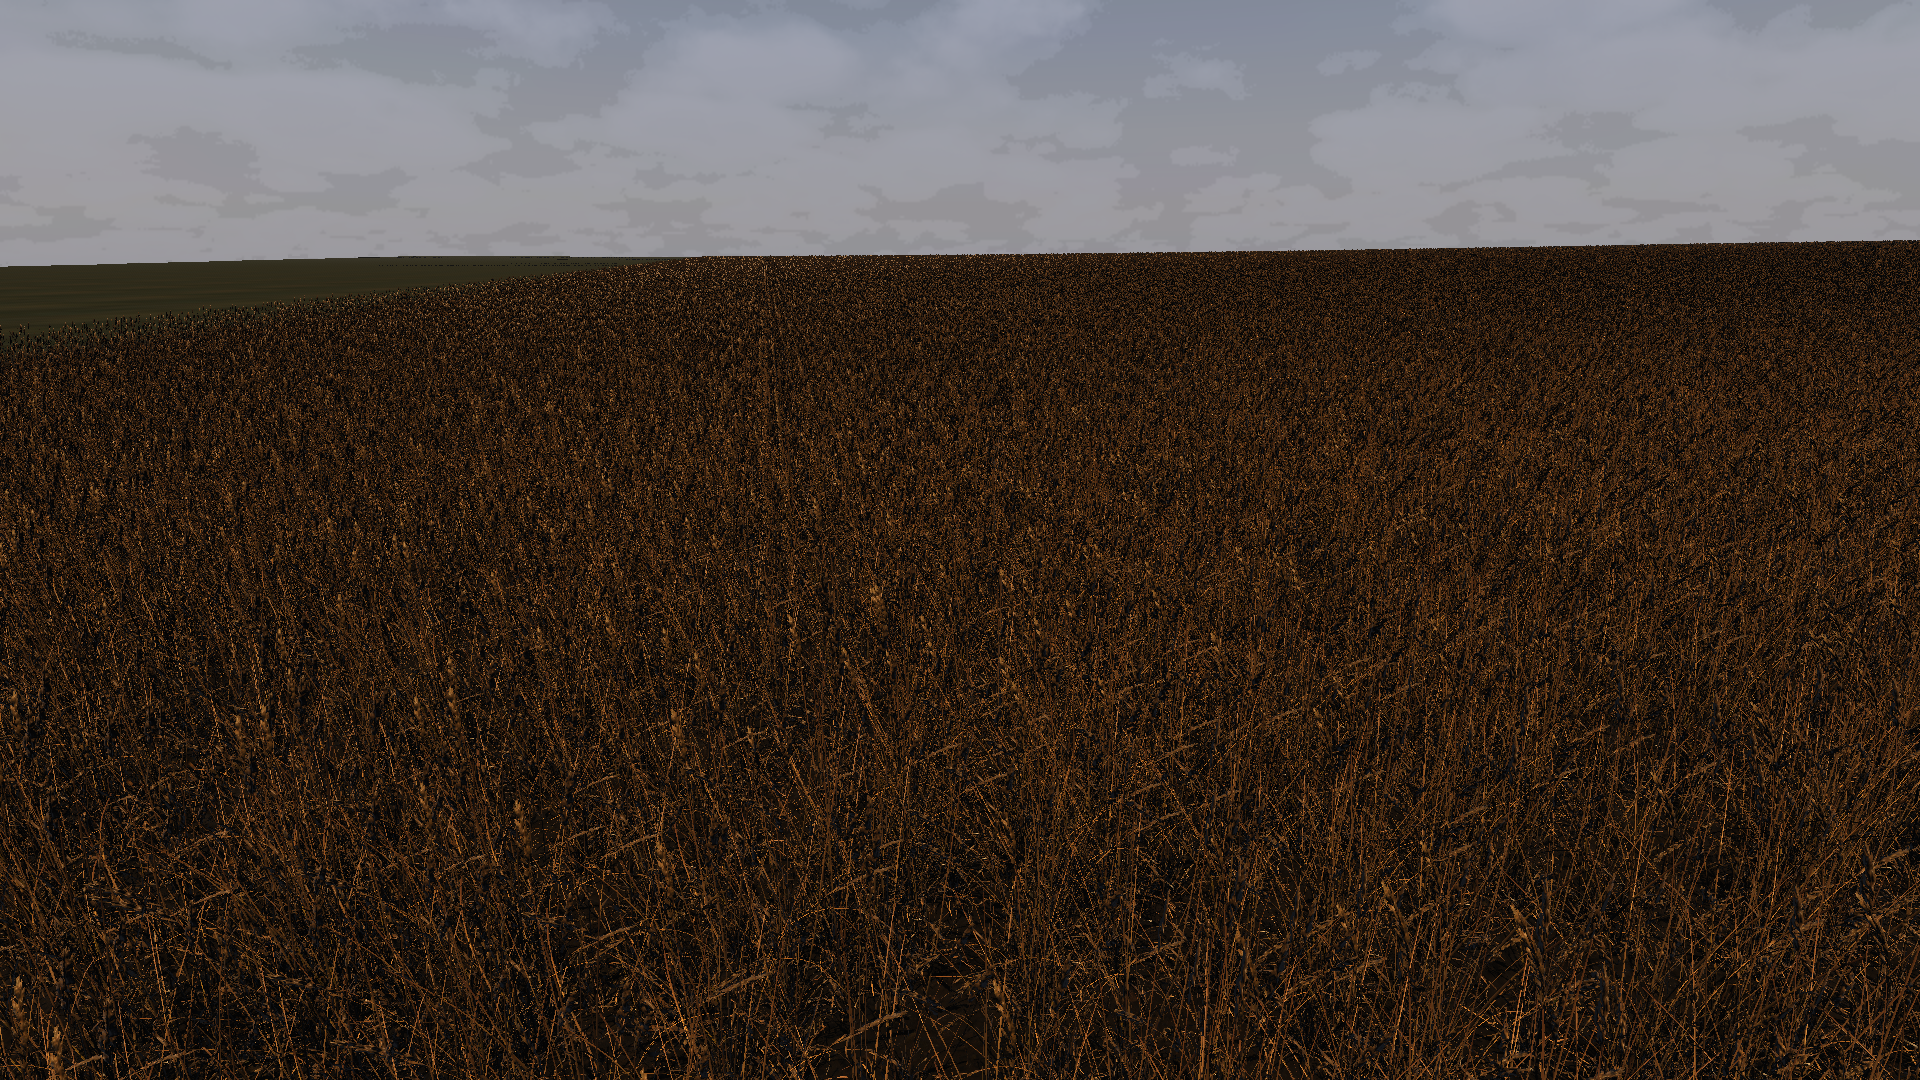
\includegraphics[width=\linewidth]{images/foggy10.png}
        \caption{Field illuminated with the SZA being set to $56^o$ and Mie Scattering Scale being increased to a non-zero value.}
        \label{fog}
    \end{subfigure}
    
    \caption{Images captured using the same SZA and different Mie Scattering Scale values. As the latter increases, simulating cloudy weather, the effects of the wheat canopy's anisotropic BRDF are mitigated, making the field appear evenly illuminated.}
    \label{notclvscl}
\end{figure}

\section{Photometric Quantities Measurement}
\label{photom-q-meas}

For the calculation of GRVI, the reflectance of a surface for the green and red bands should be calculated beforehand. As an approximation, I decided to use the reflectance formula for Lambertian surfaces in order to simplify this process. Although this contradicts the previously stated fact that a wheat field's canopy behaves as an anisotropic reflector, the error introduced during the calculation of reflectance is included in the challenges the trained models aim to address. The formula for calculating the reflectance of an ideal surface per band is:

\begin{equation}
    \rho_b = \frac{L_b \times \pi}{E_b}
    \label{lambertian}
\end{equation}

where $\rho_b$, $L_b$ and $E_b$ are the reflectance per band (dimensionless), luminance per band in nits and illuminance per band in lux, respectively. Clearly, the first step of approximating the GRVI of a studied surface was identifying consistent ways for acquiring the illuminance and luminance information from the synthetic scene.

\subsection{Acquiring Illuminance}

Illuminance is the amount of luminous flux falling onto a surface per unit area. Illuminance is commonly measured in lux. It is also measured in lux in this study, as that favors the calculation of reflectance.

In real-world applications, illuminance is usually measured using a lux meter, a type of light meter. This inspired me to use a virtual light meter within the digital twin. After finding an already developed implementation of a custom virtual light meter \cite{weiss_2025_lightmeter}, I added it to the project as a plugin and used it for approximating illuminance at every point of interest in the field.

The way this light meter works is by using an UE's Scene Capture Component actor to render radiometric linear images of a white surface, calculating the luminance of the light reflected by the surface using pixel values and, through it, calculating illuminance. A variable of the light meter actor stores the measurement. Initially, the light meter could only calculate the combined illuminance of all three channels. I modified its Blueprint to overcome this limitation and expose the illuminance of the green and red bands separately.

The placement of the light meter in the digital environment and the method employed for retaining its readings is analyzed later on.

\subsection{Acquiring Luminance} \label{findlum}

Luminance is the measure of the amount of light reflected by a surface and perceived by a sensor. In order for this information to be extracted from an Unreal Engine environment, a deeper understanding of the Unreal Engine's color rendering pipeline should be achieved.

The Unreal Engine’s color rendering pipeline, as described in UE’s documentation \cite{oztalay_2021_colorpipeline}, is displayed in Figure~\ref{cl-pp}. The first part of the pipeline is the description of the textures appearing in the scene, many of which are in the 8-bit, sRGB color space. These textures are then converted to the engine’s linear working space and, after they interact with the scene’s lighting and shading, an HDR image is produced. This is what UE’s tools refer to as Scene Color, and it expresses the rendered luminance before any kind of post-processing is applied.

\begin{figure} [htb]
    \centering
    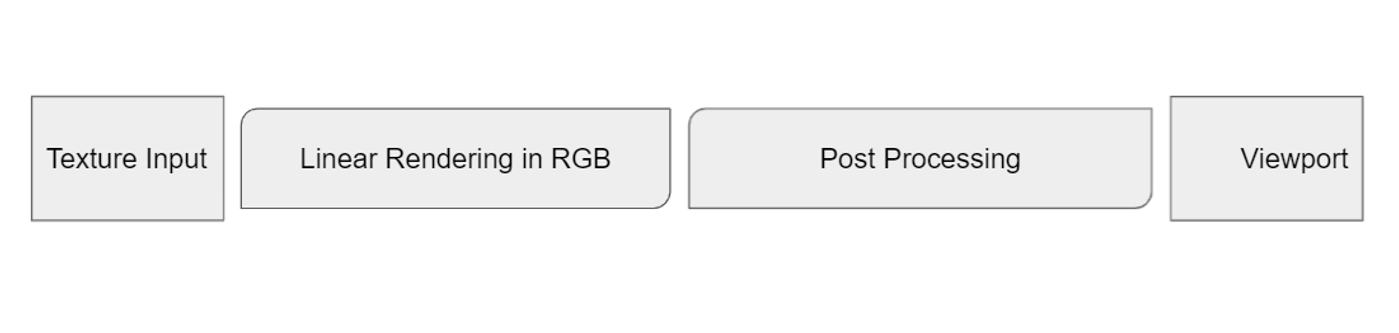
\includegraphics[width=1\linewidth]{images/color_pipe.png}
    \caption{Unreal Engine's color rendering pipeline.}
    \label{cl-pp}
\end{figure}

Post-processing includes several steps, and it is responsible for the transformation of the pixel values rendered in Scene Color to the values that appear in the viewport. The steps that are considered more relevant in the context of this study are the ones that affect the luminance as it is perceived by a sensor, and they are managed by Tonemapper. Tonemapper is a non-linear system responsible for mapping the Scene Color to a dynamic range that can be displayed to the editor’s viewport, while also applying lighting-relevant adjustments like bloom and exposure. Although tonemapping was overall observed to produce more realistic colors, compared to the ones appearing in raw Scene Color, its black-box nature affects the usability of the produced image. More importantly, the illuminance estimated from the Scene Color values, as described before, is more strongly associated with the luminance derived from Scene Color than with the color values displayed in the viewport.

For the scene luminance to be captured, an equivalent to the Cine Camera actor should be identified, capable of capturing the colors as they appear in the scene. The actor with the closest functionality to this is the Scene Capture Component (SCC) 2D. By setting SCC to capture the linear scene color, it is possible to see the pre-tonemapping colors, which are equivalent to luminance. A drawback of SCC is that it does not provide a straightforward way to save the captured images to the computer's disk, at least in an automated way. Unreal Engine does allow the user to save the captured images of the scene manually in .EXR format, with pixels representing linear luminance values, but saving images one by one is not viable. To overcome this challenge, I used an already existing actor class called Frame Capture Manager, the source code for which I found online \cite{hess_unrealimagecapture}. Its main functionality is to expose the aforementioned feature of UE that allows the user to manually save the images captured by SCC to other actors in the form of a function (void CaptureNonBlocking()), enabling the automated capturing and saving to disk of scene color images. More about the Frame Capture Manager and how it was used in this context is explained in the \hyperref[chap4]{Data Collection} chapter.

\begin{figure}[htb]
    \centering
    
    \begin{subfigure}{0.48\linewidth}
        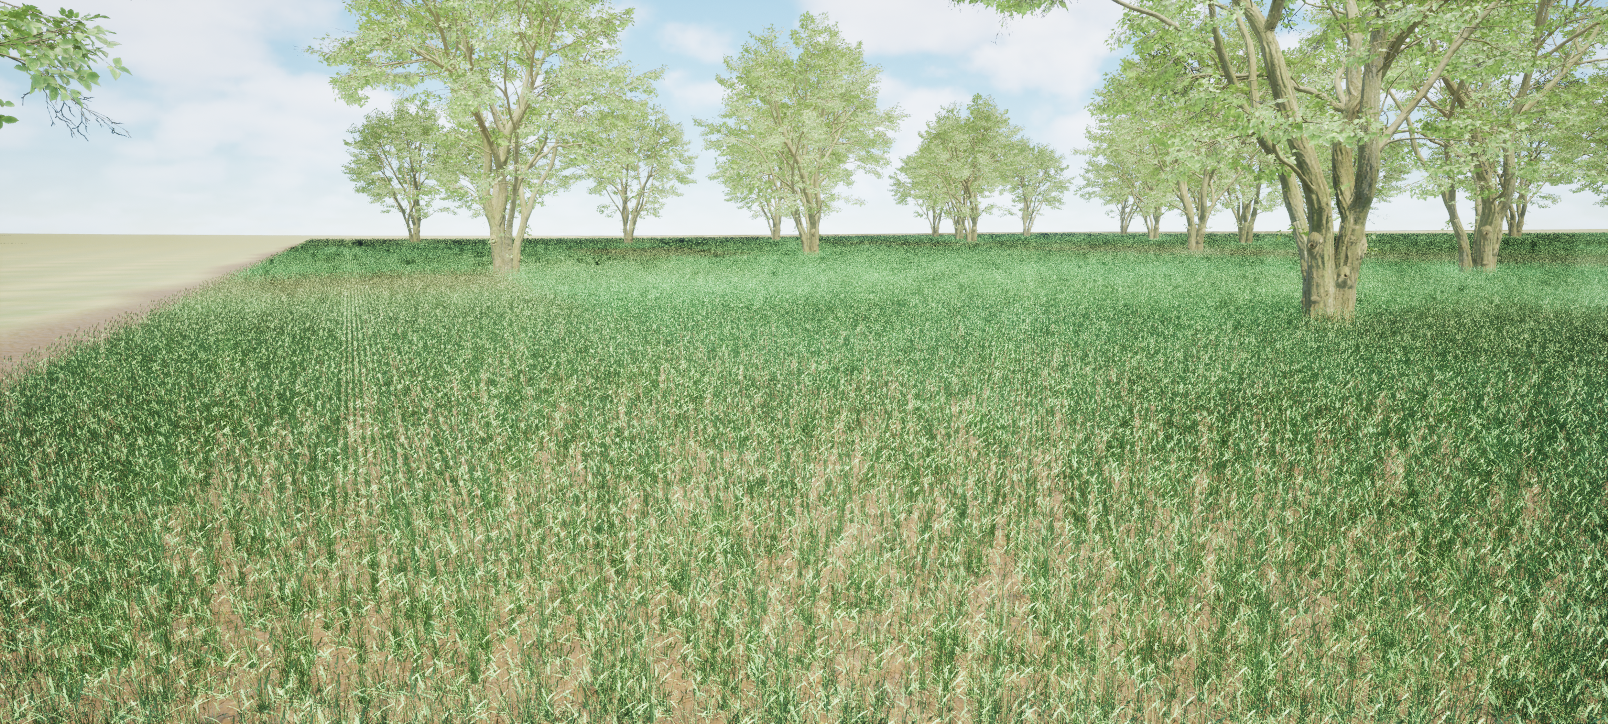
\includegraphics[width=\linewidth]{images/viewport_img.png}
        \caption{Image captured as rendered in the viewport.}
        \label{viewport}
    \end{subfigure}\hfill
    \begin{subfigure}{0.48\linewidth}
        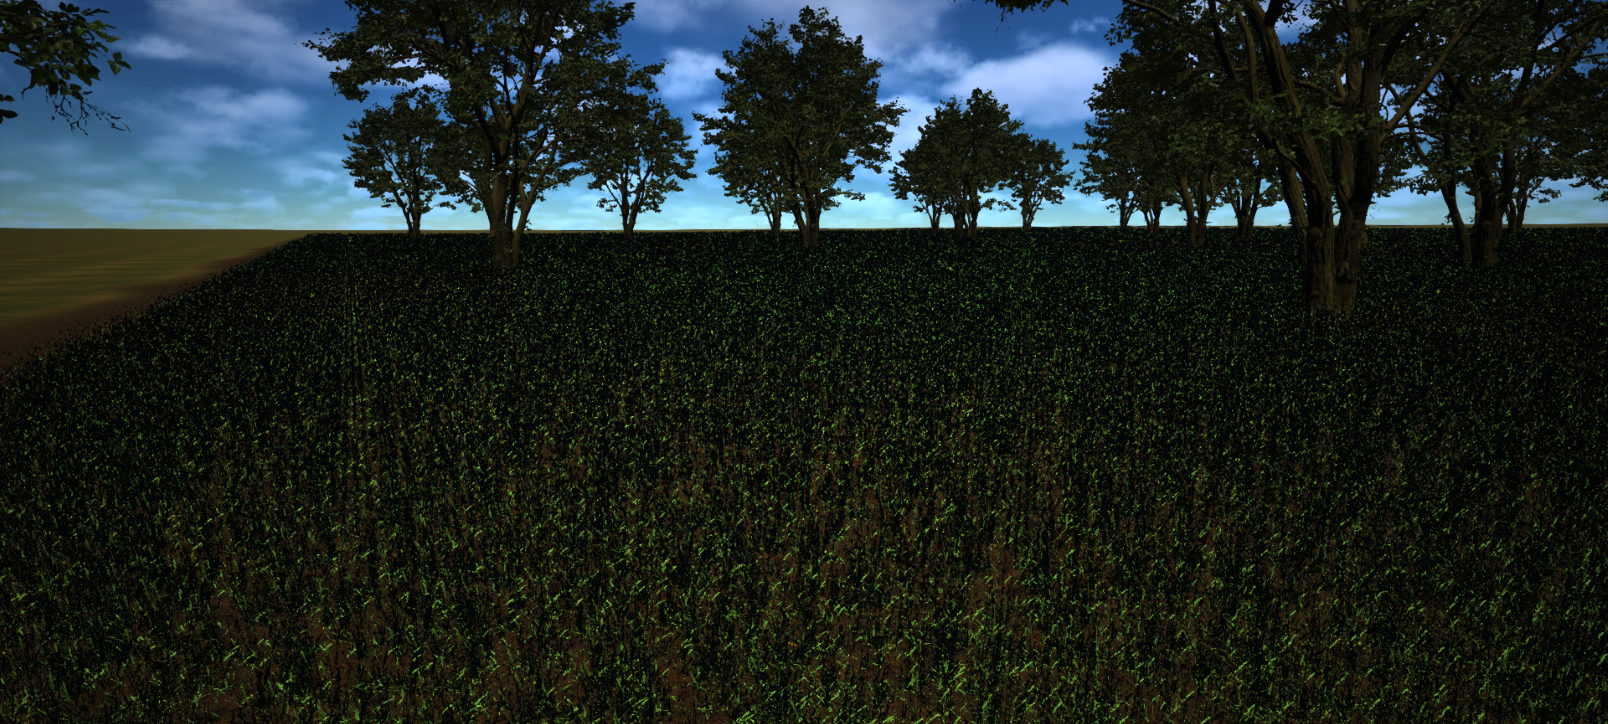
\includegraphics[width=\linewidth]{images/scc_img.png}
        \caption{Image captured using SCC.}
        \label{scc}
    \end{subfigure}
\end{figure}